\documentclass[a4paper,numbers=noenddot,abstract,DIV=calc]{scrbook} %appendixprefix=true,chapterprefix=true
\usepackage{amssymb}
\usepackage{scrpage2}
%\usepackage{xunicode}
\usepackage{fontspec}
\defaultfontfeatures{Ligatures={TeX}}
\setmainfont[Numbers=OldStyle,BoldFont={Bulmer MT Std Bold},BoldItalicFont={Bulmer MT Std Bold Italic}]{Bulmer MT Std}
\setsansfont[BoldFont={Bulmer MT Std Bold},BoldItalicFont={Bulmer MT Std Bold Italic}]{Bulmer MT Std}
%\setmainfont[Numbers=OldStyle]{Bulmer MT Std}
%\setsansfont[Numbers=Lining]{Bulmer MT Std}
%\addtokomafont{disposition}{\rmfamily \bfseries}
\setmonofont[Scale=.8]{Consolas}
\usepackage{polyglossia}
\setmainlanguage{brazil}
\setotherlanguages{french,english,german,russian,greek}
\usepackage{arabxetex}
%\newfontfamily\russianfont[Script=Cyrillic]{Minion Pro}
%\newfontfamily\greekfont[Script=Greek]{Minion Pro} 
\newfontfamily\greekfont{Minion Pro} 
\newfontfamily\russianfont{Minion Pro}
\newfontfamily\arabicfont[Script=Arabic]{Adobe Arabic}
%\usepackage{amssymb}
\usepackage[tocgraduated]{tocstyle}
\usetocstyle{nopagecolumn}
\usepackage{graphicx}
%\usepackage{chngcntr} %isso aqui tira figura 0.1... etc
%\counterwithout{figure}{chapter}%
\deffootnote[1em]{0em}{1em}{\textsuperscript{\thefootnotemark} }
%\setcounter{secnumdepth}{0}
\usepackage{eulervm}
%\setkomafont{disposition}{\sffamily}
\newfontfamily{\gr}{Minion Pro}
\usepackage{tabularx}
\usepackage{booktabs}
\usepackage{array}
\usepackage[normalem]{ulem}
\usepackage[version=3]{mhchem}
\usepackage{fixltx2e}
\usepackage{textcomp}
\usepackage[official]{eurosym}
\usepackage{wasysym}
\usepackage{multicol}
\usepackage{sidecap}
\usepackage{enumitem}
\usepackage{xeCJK}
\setCJKfamilyfont{zhrm}{SimSun}
\setCJKfamilyfont{jarm}{MS Mincho}
\setCJKfamilyfont{korm}{Batang}

\newcommand\Chinese{\renewcommand\CJKrmdefault{zhrm}\CJKnospace\normalfont}
\newcommand\Japanese{\renewcommand\CJKrmdefault{jarm}\CJKnospace\normalfont}
\newcommand\Korean{\renewcommand\CJKrmdefault{korm}\CJKspace\normalfont}

%\usepackage[tables,dvipsnames,xetex]{xcolor}
\usepackage[bookmarks]{hyperref}
\usepackage[dvipsnames]{xcolor}
\setheadsepline{.4pt}[\color{BurntOrange}]
%\setlength{\parskip}{0pt}
%\usepackage{enumerate}
%\usepackage{enumitem}
\usepackage{framed}
\definecolor{shadecolor}{Gray}{10.0}
\usepackage[xcolor]{mdframed}
\renewcommand\partpagestyle{empty}
%\setkomafont{title}{\rmfamily \bfseries}
%\addtokomafont{subtitle}{\LARGE \sffamily}
%\addtokomafont{title}{\color{gray}}
%\newcommand{\altern}[1]{{\fontspec{EB Garamond:+salt}#1}} % for long-tailed \altern{Q} etc.
%\newcommand{\alternitalic}[1]{{\fontspec{EB Garamond Italic:+salt}#1}}
%\addtokomafont{chapter}{\itshape \bfseries}
%\addtokomafont{section}{\scshape}
%\setkomafont{subsection}{\itshape}
%\addtokomafont{chapter}{\color{Red}}
%\addtokomafont{section}{\color{Bittersweet}}
\setlength{\parskip}{0pt}
%\definecolor{callunapink}{rgb}{121,16,84}
\usepackage{geometry}
\usepackage{ccicons}
\usepackage{lettrine}
\setkomafont{caption}{\sffamily}
\setkomafont{captionlabel}{\sffamily}
%\setcapindent{0pt}


%\usepackage[hyphens]{url}
%\usepackage[titletoc]{appendix}


\title{\fontsize{50}{60}\selectfont \textcolor{YellowOrange}{\rmfamily\LaTeX}}
\subtitle{\textcolor{Dandelion}{UM SISTEMA DE PREPARAÇÃO DE TEXTOS}}
\author{Youssef Cherem\thanks{\href{mailto:cherem@unifesp.br}{cherem@unifesp.br}}}
\date{MMXII}


\dedication{Dedicado a todos os amantes da tipografia.}



% %Para fonte Kepler parênteses:
%\XeTeXinterchartokenstate = 1
%\XeTeXcharclass `( 100
%\XeTeXcharclass `f 101
%\XeTeXinterchartoks 100 101 = {\kern-0.4pt}


\begin{document}

\frenchspacing


\newgeometry{top=3cm,left=3cm,right=3cm,bottom=3cm}
\maketitle

\restoregeometry

%\pagecolor{white}

%\chapter*{}
%\thispagestyle{empty}
%\phantom{}
%\vfill
%{\large \emph{Dedicado a todos os amantes da tipografia.}}
%\vfill
%\cleardoublepage

\tableofcontents

\listoffigures

\listoftables

\chapter{Introdução}

\section{O que é TeX?}
%\vspace{-2cm}
\TeX (X ou chi pronunciado como o j espanhol ou k) é uma linguagem de mark-up e de programação de baixo nível criada por Donald Knuth para diagramar documentos com uma estética agradável e estruturalmente consistentes. O nome \TeX é a primeira sílaba das palavras gregas \textgreek{τεχνολογία} (``tecnologia''), e \textgreek{τέχνη} (\textit{techni}), ``arte''.
	
Quando Knuth começou a escrever o programa de diagramação (\textit{typesetting engine}) em 1977 para explorar o potencial dos equipamentos de impressão digital que estavam começando a se infiltrar na indústria da editoração gráfica na época, esperando especialmente reverter a tendência da deterioração da qualidade tipográfica afetava seus próprios livros e artigos.

O TeX é uma linguagem de programação para diagramação de textos (typesetting). O controle fino que o TeX oferece o torna uma ferramenta muito poderosa, mas também muito difícil, consumindo muito tempo.  Mas TeX é extremamente estável, pode rodar em muitos tipos de computador, e é praticamente livre de bugs.

Baseado em linguagem \TeX, na década de 1980 Leslie Lamport criou o conjunto de macros chamado \LaTeX, que poupa tempo, automatiza certas tarefas e reduz erros, especialmente para documentos que contenham fórmulas matemáticas.

O \LaTeX{} é um software modular, composto de programas binários e conjuntos de macros chamados pacotes ou estilos, que podem ser utilizados, acrescentados e modificados. Alguns destes são empacotados com a maioria das distribuições do TeX/\LaTeX; outros podem ser encontrados no \textit{Comprehensive TeX Archive Network} (CTAN).

Como o \LaTeX{} inclui um grupo de comandos TeX, o processamento de um documento \LaTeX{} é essencialmente programação. Você cria um arquivo de texto em marcação \LaTeX. O programa ``lê" este texto marcado para produzir o documento final.
Essa abordagem tem algumas desvantagens em comparação com programas visuais como o OpenOffice/LibreOffice e o Microsoft Word©.

\section{Por que usar o \LaTeX?}

Devemos ser muito claros: você usa o processador de texto que quiser. Se quiser escrever seus textos e entregá-los com o Word, ou OpenOffice, ou Pages da Apple, ou o InDesign, da Adobe, ou GoogleDocs, para o conteúdo do seu texto isso vai fazer pouca diferença. Mas se você quer uma aparência profissional, usa muitas figuras ou fórmulas matemáticas, está escrevendo uma tese um ou texto técnico ou acadêmico, o resultado final, com o mesmo nível de esforço, vai ser muito diferente. No começo o \LaTeX{} parece muito difícil, mas facilita e automatiza muito tarefas complexas, e a maioria dos comandos é bem intuitiva. Na verdade, ele não passa de um conjunto de macros para geração de texto. E, uma vez que você personaliza um modelo, você simplesmente ``joga" qualquer texto nele que ele sai com a aparência desejada. Com os outros programas, acontece o oposto: você tem mais liberdade, deve saber muito bem o que está fazendo. O \LaTeX{}, na verdade, faz o trabalho do diagramador ou designer gráfico para você.

%Você pega um modelo, geralmente mal feito, ou faz um do jeito que você acha que vai ficar bom baseado na aparência da tela, e aí você tenta criar uma tabela de conteúdo, que vai ficar mais ou menos, justificar o texto, colocar índices de figuras, de tabelas, legendas nas tabelas e figuras, numerar as tabelas e figuras, numerar as equações (isso só tem jeito de fazer à mão no Word)\ldots{} e, quando chega a hora, colocar os cabeçalhos e rodapés com números de página ou correntes (refletindo o capítulo ou seção), cortar seções e começar numeração romana (antes do primeiro capítulo) e arábica (a partir do primeiro capítulo), inserir referências --- aí sim você vai sentir a diferença.

%Por outro lado, eu não vou ser radical e dizer que você deve ou precisa de usar esta ferramenta. Provavelmente você não precisa; você não é físico, nem matemático, nem engenheiro; você não está escrevendo uma tese, você não é nerd, não vai perder tempo com firulas, e por aí vai. No Brasil quase nenhuma publicação acadêmica aceita esse formato. 

Contudo, você não precisa, necessariamente, usar esta ferramenta. Devo deixar claro que, no Brasil, praticamente nenhuma publicação aceita esse formato. Mas temos que salientar que o resultado é profissional, para impressão: compare um livro bem produzido e um artigo acadêmico pobremente formatado no Word: o \LaTeX{} é a maneira mais fácil e barata de produzir textos que mais se aproximam de revistas e livros compostos com um profissional (muito bem) pago para cuidar da aparência do seu material. 

Porém, o \LaTeX{} tem alguns inconvenientes:
 
\begin{itemize}

\item você geralmente não vê a versão final do documento quando está editando;
\item você geralmente precisa de conhecer os comandos de marcação;
\item pode ser difícil dar um visual muito personalizado aos documentos.
\end{itemize}

Por outro lado, há certas vantagens na abordagem \LaTeX:
\begin{itemize}
\item o programa é de graça, de código aberto, com manuais que explicam praticamente tudo;
\item os documentos originais podem ser lidos em qualquer editor de texto;
\item você pode se concentrar exclusivamente na estrutura e no conteúdo do documento, sem ficar perdido em questões superficiais de layout;
\item você não precisa de ajustar manualmente as fontes, o tamanho do texto, espaçamento e divisão de linhas para legibilidade: o \LaTeX{} cuida disso automaticamente;
\item o layout, as fontes, as tabelas etc. são consistentes no documento todo;
\item fórmulas matemáticas podem ser escritas com facilidade;
\item índices, notas de rodapé, citações e referências são geradas com facilidade.
\item você é forçado a estruturar seus documentos corretamente.
\end{itemize}



\section{Como o \LaTeX{} funciona}
 
 \begin{enumerate}
 \item  Você digita um texto \item faz as marcações necessárias (indicando título, capítulo, seções, ênfases etc.) \item  roda o programa para gerar o produto final (um texto diagramado em .pdf ou outros formatos menos usuais).
 \end{enumerate}


Para isso, você precisa de, no mínimo, uma distribuição (uma versão do programa) e um editor de textos específico,  (para facilitar a digitação e compilação do texto), além de um leitor de pdfs (Acrobat Reader ou similares).

%\section{Outras distribuições \TeX}
%Ao procurar informações sobre \LaTeX, você pode se deparar com nomes como  XeTeX, ConTeXt, LuaTeX e outros com o sufixo \TeX. Alguns são programas, outros, distribuições. Na verdade você não precisa de se preocupar com isso: basta apenas saber que o Xe\LaTeX{} é um programa que permite usar caracteres Unicode e possibilita uso de fontes comuns que você tem em seu computador (formatos .ttf e .otf).


\section{Instalando o programa (uma ``distribuição")}
\label{distribuicoes}
Há dois tipos básicos de distribuição:
\begin{description}
\item [TeX Live] (\url{ http://www.tug.org/texlive/}) para Linux, Mac  (\url{ http://www.tug.org/mactex}) e Windows. No Linux, pode instalar a partir da linha de comando (por exemplo, no Ubuntu: \texttt{sudo apt-get install texlive-full}), ou através do gerenciador de pacotes. 
\item[MiKTeX]  (\url{ http://www.miktex.org}) para Windows.

\end{description}

\section{Instalando um editor de textos}
Há muitos por aí. Na verdade, você pode editar seus textos no Notepad ou até mesmo no Word ou no OpenOffice/LibreOffice.  Eu vou citar apenas alguns.

\begin{description}

\item[Texworks] \url{http://www.tug.org/texworks/}.Vem com MiKTeX e com Texlive para Windows e Mac; no Linux tem que instalar separadamente. 

\item [TexShop] (\url{http://pages.uoregon.edu/koch/texshop/}), para Mac, vem com MacTeX.

\item [Kile] \url{http://kile.sourceforge.net/}
É um editor para o ambiente gráfico KDE do Linux.

\item [TeXmaker] \url{http://www.xm1math.net/texmaker/}
É um editor útil multiplataforma com seu próprio leitor de pdfs.

\item  [TeXStudio] (\url{texstudio.sourceforge.net/})
Muito semelhante ao TeXmaker, aceita também correção ortográfica (o mesmo dicionário do OpenOffice). Tem também uma grande quantidade de símbolos matemáticos e funções de autocompletar que agilizam a criação do texto.

\end{description}

\chapter{Criando um texto básico}

Um arquivo .tex tem basicamente duas partes: o \textit{preâmbulo}, que vem antes do texto e define aspectos como tamanho da letra, aparência, layout das margens e tamanho da página, e o \textit{texto} propriamente dito.

A melhor forma de aprender o \LaTeX{} é testando e observando o código (o arquivo original antes de ser compilado/diagramado). Aqui veremos como criar um artigo simples. Programas como o TexStudio, que foi utilizado para compor este texto, contêm preâmbulos pré-definidos, que, com algumas alterações, podem ser usados para compor um texto em português com o mínimo de esforços. Mas é claro que você pode adicionar seu toque pessoal, à medida em que você for aprendendo. Aqui veremos um exemplo básico, então não vamos nos preocupar com fontes (tipos de letras) ainda. No entanto, valem algumas considerações iniciais.

%Espaços maiores que um espaço são desconsiderados (mas há comandos para criar espaços maiores). Para passar para outro parágrafo, o comando é: \textbackslash\textbackslash{} ou duas vezes ENTER. (Se teclar mais que duas vezes o enter o resultado será o mesmo.)
%
%Para inserir caracteres acentuados diretamente, como em português, basta inserir \begin{verbatim}\usepackage[utf8]{inputenc}\end{verbatim} 
%ou \begin{verbatim}\usepackage[latin1]{inputenc}\end{verbatim} 
%no preâmbulo.
%
%Para inserir um travessão, use três traços: \verb+---+, e para separar números ou datas, use \verb+--+ (significando: ``de -- até").
%
%Para aspas inglesas, use: \verb+``+ para abrir e \verb+"+ para fechar aspas.
%
%Os delimitadores de seção, capítulo etc. seguem o seguinte padrão:\begin{verbatim}\documentclass[OPÇÕES]{ESTILO DO DOCUMENTO}\end{verbatim} (se é livro [book], relatório[report], artigo [article], documento segundo ABNT [abnt], carta [letter] etc etc.). E os pacotes (conjunto de macros) que ``fazem" as coisas para você são: \begin{verbatim}\usepackage[OPÇÕES]{PACOTE}\end{verbatim} Por exemplo, \begin{verbatim}\usepackage{hyperref}\end{verbatim} insere referências que você pode clicar para navegar no documento (clicando numa entrada no sumário) ou abrir uma página na internet.

Vejamos agora como fica um texto básico, tirado da Wikipedia:

\begin{verbatim}
\documentclass[12pt,a4paper]{article}
\usepackage[brazil]{babel}
\usepackage[utf8]{inputenc}
\usepackage[T1]{fontenc}

\title{O Sistema \LaTeX}

\begin{document}

\maketitle

A ideia central do \LaTeX\ é distanciar o autor
o máximo possível da apresentação visual da informação.

Ao invés de trabalhar com ideias visuais, o usuário é
encorajado a trabalhar com conceitos mais lógicos --- e,
consequentemente, independente da apresentação --- como capítulos,
seções, ênfase e tabelas, sem contudo impedir o usuário da
liberdade de indicar, expressamente, declarações de formatação.
 
A versão mais recente é a \LaTeXe.
 
% Isto é um comentário que não será processado. Ele serve apenas
% para fazer anotações não incluídas no resultado final. Atenção
% ao símbolo do comentário: porcentagem (%).
A seguir, a fórmula das combinações como um exemplo simplório
da capacidade matemática do \LaTeX:
 
\begin{eqnarray}
C_k^n &=& \frac{n!}{k!(n-k)!}
\end{eqnarray}
 
\end{document}
\end{verbatim}


Isso vai ter a aparência da figura \ref{latexbasico}.

\begin{figure}
\centering
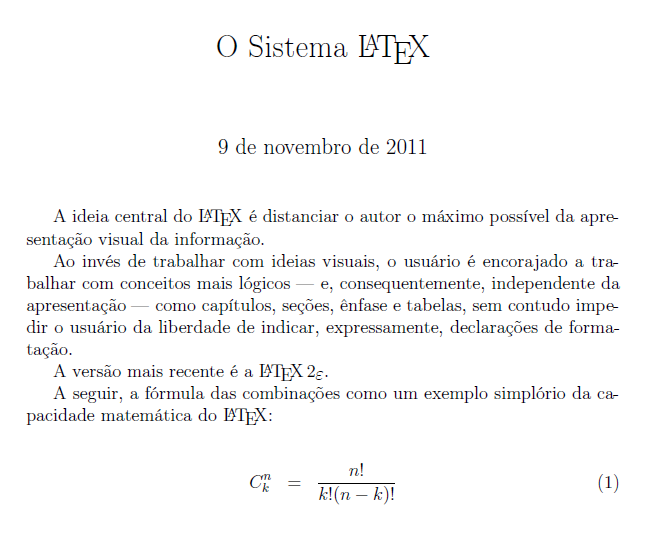
\includegraphics[width=0.6\textwidth]{latexbasico.png}
\caption{Um texto simples.}
\label{latexbasico}
\end{figure}

No caso, tudo o que eu precisei de fazer foi rodar o comando \verb+pdflatex latexbasico.tex+ na pasta onde deixei o arquivo \verb+latexbasico.tex+ ou então apertar o botão \verb+pdflatex+ no menu do editor para gerar um arquivo \verb+pdf+ de mesmo nome. Depois é só abrir o \verb+pdf+ e ver como ficou.

\section{Comandos}
Os comandos em \LaTeX{} são sensíveis a maiúsculas e minúsculas, e têm um dos dois formatos:

\begin{itemize}
\item Começam com um \textbackslash{} e têm um nome composto só de letras. Nomes de comando são terminados por um espaço, por um número ou qualquer outro caractere que não é letra.
\item Consistem de um \textbackslash{} e exatamente um caractere não alfabético.
\end{itemize}

\section{Ambientes \LaTeX}
Os \textit{ambientes} têm um papel semelhante a comandos, mas geralmente afetam só uma parte específica do documento. Sua sintaxe é:

\begin{verbatim}
\begin{NOME DO AMBIENTE}
Texto a ser influenciado
\end{NOME DO AMBIENTE}
\end{verbatim}

Entre \verb+\begin+ e \verb+\end+ você pode colocar outros comandos e outros ambientes. Tudo no \LaTeX{} pode ser expresso em termos de comandos e ambientes.


\section{Caracteres especiais}
\label{caracteres}

Vocês devem ter notado que alguns caracteres são usados para os comandos do \LaTeX:

\begin{verbatim}
# $ % ^ & _ { } ~ \
\end{verbatim}

O que fazer, então, quando quisermos que eles apareçam no texto? Geralmente colocamos uma barra à esquerda, ou outros comandos quando o caso é a própria barra à esquerda (que se usarmos duas, gera um novo parágrafo) ou o acento circunflexo:

\begin{center}
\begin{tabular}{cc}
\verb+\#+ & \# \\
\verb+\$+ & \$ \\ 
\verb+\%+ & \% \\ 
\verb+\textasciicircum{}+ & \textasciicircum{} \\ 
\verb+\&+ & \& \\ 
\verb+\_+ & \_ \\ 
\verb+\{ \}+ & \{ \} \\ 
\verb+\~{} + & \~{} \\ 
\verb+\textbackslash{}+ & \textbackslash{} \\ 

\end{tabular} 
\end{center}

\section{Comentários}
Podemos escrever um texto, ``comentando" o original, mas esse comentário não aparecerá no texto compilado. Para isso, usamos \verb+%+.

\section{Espaços, acentos e pontuação}

Espaços maiores que um espaço são desconsiderados (mas há comandos para criar espaços maiores). Para começar outro parágrafo, tecle duas vezes \textsf{ENTER} ou \textbackslash\textbackslash{}. (Se teclar mais que duas vezes o enter o resultado será o mesmo.)
\label{espacos}

Para inserir caracteres acentuados diretamente, como em português, basta inserir \begin{verbatim}\usepackage[utf8]{inputenc}\end{verbatim} 
ou \begin{verbatim}\usepackage[latin1]{inputenc}\end{verbatim} 
no preâmbulo.
\label{acentos}

Para inserir um travessão (---), use três traços: \verb+---+, e para separar números ou datas, use \verb+--+ (significando: ``de -- até").

Para aspas inglesas, use: \verb+``+ para abrir e \verb+"+ para fechar aspas.

%\section{A estrutura do arquivo}
%
%Todo arquivo .tex começa com o tipo de documento que queremos criar:
%
%\begin{verbatim}
%\documentclass{...}
%\end{verbatim}
%
%Depois podemos incluir comandos que influenciam o estilo do documento como um todo:
%
%\begin{verbatim}
%\usepackage{...}
%\end{verbatim}
%
%Finalmente, podemos começar o documento com
%
%\begin{verbatim}
%\begin{document}
%\end{verbatim}
%
%e encerrar com:
%
%\begin{verbatim}
%\end{document}
%\end{verbatim}

%Tudo o que fica antes de \verb+\begin{document}+ é chamado de \textit{preâmbulo}.

\section{Classes de documentos}

A primeira informação que o \LaTeX{} precisa de saber ao processar um arquivo e o tipo de documento que o autor quer criar. Isso é especificado usando o comando \verb+\documentclass{...}+.

A classe é o tipo de documento que deve ser criado. A distribuição \LaTeX{} fornece classes adicionais para outros documentos, incluindo cartas e slides. Os parâmetros opcionais personalizam o comportamento da classe, e estão entre colchetes, devendo ser separados por vírgulas.

Exemplo: um arquivo de entrada (input) pode começar com:

\begin{verbatim}
\documentclass[11pt,twoside,a4paper]{article}
\end{verbatim}

Que significa: o documento é um artigo, com fonte básica de tamanho de 11 pontos (\texttt{11pt}), página frente e verso (\texttt{twoside}) e papel A4.

Algumas outras classes são: \texttt{book} (livro), \texttt{report}, \texttt{abntex2} (formato ABNT), \texttt{beamer} (para apresentações de slides). Outras opções podem ser vistas na tabela \ref{tab:classes}.

\begin{table}
\caption{Principais opções das classes padrão do \LaTeX}
\label{tab:classes}
\begin{tabularx}{\textwidth}{XX}
\toprule
 10pt, 11pt, 12pt & Tamanho da fonte principal do documento. Geralmente o tamanho padrão das classes é 11pt \\ 
 a4paper, letterpaper, a5paper, legalpaper, executivepaper\ldots & Tamanho do papel. Geralmente vem com A4, se não for especificado. \\ 
 fleqn & Fórmulas alinhadas à esquerda. \\ 
 leqno & Número da fórmula à esquerda. \\ 
 titlepage, notitlepage & Especifica se vai ter ou não página separada para o título. A classe article não tem, por padrão; report e book, têm. Se quiser mudar esse comportamento padrão, deve indicar \\ 
 onecolumn, twocolumn & Uma ou duas colunas. \\ 
 twoside,oneside & twoside=frente e verso, padrão em livros; oneside=só frente, padrão em article e report. \\ 
 landscape & página na horizontal \\ 
 openright,openany & Começa novos capítulos com páginas da direita (openright) ou qualquer página (openany). Padrão para livros: openright. \\ 
 draft & Esboço. Indica problemas de hifenização e justificação com um pequeno quadrado na margem para ser localizado.  \\ 
\bottomrule
\end{tabularx}
\end{table}

Por exemplo, se quiser escrever um relatório com fonte 12 pontos em A4, em modo de esboço, você usaria:

\begin{verbatim}
\documentclass[12pt,a4paper,draft]{report}
\end{verbatim}

\section{Pacotes}
\label{pacotes}
Ao escrever um documento, você vai perceber que provavelmente há algumas áreas em que o básico não vai resolver seu problema. Se quiser colocar figuras, texto colorido, fontes, personalizar margens, você vai precisar de ``melhorias". Essas melhorias são chamadas de ``pacotes". Eles são ativados com o comando

\begin{verbatim}
\usepackage[opções]{pacote}
\end{verbatim}

em que ``opções'' são palavras chave que ativam características especiais do pacote e ``pacote" é o nome do pacote. A maioria das distribuições atuais vêm com muitos pacotes e classes, mas mesmo assim é possível instalá-los manualmente. O Miktex tem uma opção de instalar automaticamente pacotes que faltam (se estiverem disponíveis nos servidores), e o Texlive também tem uma função semelhante (ver os sites da seção \ref{distribuicoes} na página  \pageref{distribuicoes}). Uma maneira mais fácil é colocar estilos baixados da internet (com extensões .sty para pacotes e .cls para classes) na mesma pasta em que está o documento a ser processado, mas isso tem o inconveniente de que só documentos naquela mesma pasta poderão usar os estilos. Para instalar no sistema, quando estamos usando Texlive, podemos criar uma pasta chamada \texttt{texmf} no diretório do usuário \verb+~/[NOME DO USUÁRIO]+ no Linux ou \verb+C:\Users\[NOME DO USUÁRIO]+ no Windows. Então, vamos até essa pasta no prompt de comando e digitamos: \texttt{texhash texmf}. É assim que podemos instalar, com o Texlive, o estilo ABNT no Windows ou Linux.(Ver a página do ABNTeX2 em: \url{http://code.google.com/p/abntex2/}.)

% Primeiro baixe o estilo (\url{http://sourceforge.net/apps/mediawiki/abntex/index.php?title=Main_Page})(no Linux também temos a opção mais confortável de instalar automaticamente através da linha de comando--- \texttt{sudo apt-get install abntex}--- ou via gerenciador de pacotes) e extraia em qualquer lugar. Depois copie a pasta \texttt{texmf} para seu diretório de usuário (ver acima), abra um prompt de comando (\texttt{cmd} no Windows) e digite: \texttt{texhash texmf}. Se o sistema for MAC, copie o que está dentro da pasta texmf para /usr/local/texlive/texmf-local e rode o comando sudo texhash (pedirá senha). Para instalar o estilo ABNT com o Miktex no Windows a coisa é um pouco mais complicada: copie o \textit{conteúdo} da pasta \texttt{texmf} (as subpastas: bibtex\texttt{bibtex},\texttt{doc}, \texttt{makeindex}, \texttt{tex}) para a pasta de instalação do Miktex (geralmente em «Arquivos de programas»), depois vá em: Todos os programas, Miktex, Settings (Admin), na aba GENERAL, clique em REFRESH FNDB para atualizar o banco de dados.
%

\chapter{A estrutura do documento}

O principal objetivo de um texto é transmitir ideias, informação ou conhecimento ao leitor. O leitor entenderá melhor o texto se essas ideias forem bem estruturadas, e verá e sentirá essa estrutura melhor se a forma tipográfica refletir a estrutura lógica e semântica do conteúdo.

O \LaTeX{} é diferente de outros sistemas de diagramação, já que você só precisa de informar a estrutura lógica e semântica do texto. Então, o programa deriva a forma tipográfica de acordo com as ``regras" dadas na classe do documento e nos vários estilos, permitindo ao usuário estruturar seu documento de acordo com várias construções hierárquicas, incluindo capítulos, seções, subseções e parágrafos.

\section{O ambiente \texttt{document}}

Depois da declaração da classe do documento, o texto de seu documento encontra-se entre dois comandos que identificam o começo e o fim do documento propriamente dito:

\begin{verbatim}
\documentclass[a4paper]{report}

\begin{document}
 ...
\end{document}
\end{verbatim}

Os três pontos indicam onde você coloca o texto. A razão para marcar o começo do texto permitir configurações extras (ver a linha branca no exemplo acima: vamos utilizá-la em breve).

\section{Preâmbulo}
O \textit{preâmbulo} é tudo entre o começo do arquivo-fonte até \verb+\begin{document}+. Normalmente contém comandos que afetam todo o documento.

\begin{verbatim}
% simple.tex - Um artigo simples para ilustrar a estrutura do documento.

\documentclass{article}
\usepackage{mathptmx}
\usepackage[brazil]{babel}
\usepackage[utf8]{inputenc}

\begin{document}
\end{verbatim}

A primeira linha, iniciada com \%, é um comentário (não vai aparecer no texto final). O comando \verb+\documentclass+ indica o tipo de documento que queremos produzir.
O pacote \texttt{babel} serve para indicar as línguas usadas (no caso, \texttt{brazil} = português do Brasil).  \verb+\usepackage[utf8]{inputenc}+ indica uso de caracteres acentuados diretamente e \verb+\usepackage{mathptmx}+ indica o uso da fonte Times ao invés da fonte padrão do \LaTeX, que é a Computer Modern (trataremos as fontes na seção \ref{fontes} mais adiante).

Todos os ``pacotes'' que serão tratados daqui em diante, devem ser inseridos no preâmbulo (isto é, antes de \verb+\begin{document}+). Assim, para usar o pacote \texttt{enumitem} (ver página \pageref{enumitem}), devemos inserir no preâmbulo: \verb+\usepackage{enumitem}+.


\section{O cabeçalho}
No começo da maioria dos documentos haverá informação sobre o próprio documento: título, data, autor(es) etc. 

Um exemplo simples:

\begin{verbatim}
\documentclass[12pt,a4paper]{report}

\begin{document}
\title{Como estruturar um documento em \LaTeX{}}
\author{Fulano de Tal}
\date{Dezembro de 2012}
\maketitle
\end{document}
\end{verbatim}

Os comandos \verb+\title+, \verb+\author+ e \verb+\date+ são autoexplicativos. Se não for indicada a data, aparecerá o dia em que o documento foi composto. Você sempre termina o cabeçalho com \verb+\maketitle+, indicando que você terminou o cabeçalho e que ele pode ser diagramado de acordo com a classe (estilo) que você escolheu. Se você omitir \verb+\maketitle+, essas informações não aparecerão (a não ser que você as escreva manualmente).

Aqui temos um exemplo mais complicado:

\begin{verbatim}
\title{Como estruturar um documento em \LaTeX{}}
\author{Fulano de Tal\\
   Escola de Computação\\
   Universidade Tal,\\
   São Paulo,\\
   Brasil,\\
   \texttt{fulanodetal@universidadetal.br}}
\date{\today}
\maketitle
\end{verbatim}

Como pode ver, pode usar os argumentos \verb+\title+ e os outros. A barra dupla à esquerda ($\backslash\backslash$) é o comando para forçar uma quebra de linha. O \LaTeX{} normalmente decide por si só onde quebrar uma linha, e geralmente está certo, mas às vezes você precisa de terminar uma linha antes do fim, como aqui, e começar uma nova. No exemplo, na última linha, usamos uma fonte monoespaçada (de máquina de escrever) com o comando \verb+\texttt{}+, para escrever o e-mail. O comando \verb+\today+ será substituído pela data do dia, mas você pode colocar a data que quiser, sem ordem específica. Esses comandos do cabeçalho também não têm ordem específica (título, autor, data), eles serão processados de acordo com o estilo.

Se houver dois autores, pode-se separá-los com o comando \verb+\and+: 


\begin{verbatim}
\author{Fulano de Tal \and Sicrano de Tal}
\end{verbatim}


\section{Abstract/Resumo}

Como a maioria dos artigos científicos têm um resumo (e um abstract em inglês, caso a língua original não seja esta), há comandos predefinidos para compor um abstract. O comando \texttt{abstract} está
disponível nas classes \texttt{article} e \texttt{report}, mas não em \texttt{book}.

\begin{verbatim}
\begin{abstract}
Escreva seu resumo aqui
 ...
\end{abstract}
\end{verbatim}

Para escrever o resumo (em português, por exemplo) e também o abstract (em inglês), você tem duas opções. Se estiver usando o pacote \texttt{babel}, através do comando 

\begin{verbatim}
\usepackage[english,brazil]{babel}
\end{verbatim}



A língua ativada é sempre a última (no caso, brazil=português do Brasil). Você pode copiar esse código e salvar como um arquivo .tex, e fazer o teste você mesmo rodando o comando pdflatex (nome do arquivo).tex.:

\begin{verbatim}
\documentclass{article}
\usepackage[english,brazil]{babel}
\usepackage[utf8]{inputenc}
\usepackage[T1]{fontenc}
\usepackage{utopia}

\title{Um texto qualquer}
\author{Fulano de Tal}

\begin{document}

\maketitle

\begin{abstract}
Um resumo em português.
\end{abstract}

\begin{otherlanguage}{english}

\begin{abstract}
This is an abstract in English.
\end{abstract}

\end{otherlanguage}

\end{document}

\end{verbatim}

%Observação: o pacote \texttt{abntex} tem os ambientes prontos: \texttt{abstract} (para inglês) e \texttt{resumo} (para português).

A outra opção é se estiver utilizando o pacote \texttt{polyglossia}:

%\begin{framed}
 \begin{verbatim}
\documentclass{article}
\usepackage{fontspec}
\setmainfont{Minion Pro}
\setsansfont{Myriad Pro}
\setmonofont{Courier}
\usepackage{polyglossia}
\setmainlanguage{brazil}
\setotherlanguages{french,english,german,norsk}
\end{verbatim}
%\end{framed}

Abstract em inglês:

\begin{verbatim}
\begin{english}
\begin{abstract}
This is an abstract in English.
\end{abstract}
\end{english}
\end{verbatim}




\section{Comandos de seção}
Os comandos para quebra de seção são bem intuitivos. Claro que alguns comandos são apropriados a diferentes classes de documentos.

Aqui temos um exemplo simples:

\begin{verbatim}
\section{Título da Seção}

\section{Outra seção}

\subsection{Uma subseção}
\end{verbatim}

Note que não é necessário especificar números de seção, o \LaTeX{} fará isso para você. Você também não precisa de marcar o começo e o fim de uma seção. O \LaTeX{} dá 7 níveis de seção:

\begin{table}[h!]
\caption{Comandos de seção}
\label{secoes}
\begin{tabular}{lcl}
\toprule
\centering
\textbf{Comando} & \textbf{Nível} & \textbf{Comentário}\\
\verb+\part{PARTE}+ & -1 & não em cartas\\
\verb+\chapter{CAPÍTULO}+ & 0 & somente livros e relatórios\\
\verb+\section{SEÇÃO}+ & 1 & \\
\verb+\subsection{SUBSEÇÃO}+ & 2 &\\
\verb+\subsubsection{SUBSUBSEÇÃO}+ & 3 &\\
\verb+\paragraph{PARÁGRAFO}+ & 4 &\\
\verb+\subparagraph{SUBPARÁGRAFO}+ & 5 &\\
\bottomrule
\end{tabular}
\end{table}

Todos os títulos são acrescentados automaticamente ao sumário (table of contents), se você decidir inserir um. Mas se você fizer mudanças manuais de estilo no seu cabeçalho, por exemplo, um título muito longo, ou quebras de linha, ou uso incomum de fontes, isso também aparecerá no sumário --- o que você provavelmente não quer. O \LaTeX{} lhe permite criar uma versão opcional extra que só será utilizada no sumário e no topo de página (se houver). Essa alternativa é colocada entre colchetes:

\begin{verbatim}
\section[título curto]{título longo}
\end{verbatim}


\subsection{Numeração de seções}
O \LaTeX{} numera automaticamente as seções. Partes têm numerais romanos (Parte I, Parte II), capítulos e seções, numeração decimal, e apêndices, alfabética (A, B, C etc.). Você pode mudar a numeração, de acordo com a tabela \ref{secoes}. Assim, se você quiser numerar até as seções, mas não as subseções: 

\begin{verbatim}
\setcounter{secnumdepth}{1}
\end{verbatim}

Se você quiser uma seção/capítulo etc. não numerada que não vai aparecer no sumário, coloque um asterisco antes da chave:

\begin{verbatim}
\chapter*{Introdução}
\end{verbatim}

Se você quiser que essa seção não numerada apareça no conteúdo/sumário, faça o seguinte:


\begin{verbatim}
\chapter*{Introdução}
\addcontentsline{toc}{chapter}{Introduction}
\end{verbatim}




\section{Apêndices}
O comando \verb+\appendix+ indica que os capítulos ou seções devem ser numerados como apêndices:

\begin{verbatim}
\appendix
\chapter{Primeiro apêndice}
\end{verbatim}

\section{Sumário}
\label{sumario}
Todos os cabeçalhos numerados automaticamente vão para o sumário. Você não precisa de ter um, mas se quiser, é só adicionar o comando \verb+\tableofcontents+ onde quiser que apareça o sumário (geralmente depois do abstract). 

Os comandos \verb+\listoffigures+ e \verb+\listoftables+ geram, respectivamente, uma lista das figuras e uma lista das tabelas.

\chapter{Bibliografia}
\label{bibliografia}
A bibliografia, é uma das partes essenciais (e mais trabalhosas e, talvez, mais pedantes) de um texto científico ou acadêmico. Existem centenas de estilos de citação e bibliografia. O \LaTeX{} pode compor/gerar a bibliografia para você, com alguns comandos específicos (bibtex) e depois que você tiver um arquivo separado (.bib) para gerar essa bibliografia. %Gerar um arquivo desses à mão, ou mesmo pegar da Internet já no formato bibtex, e depois compilar várias vezes para ver o resultado, muitas vezes (na maioria das vezes) não vale a pena. %Mas se você quiser se aventurar, é só acessar: \url{http://en.wikibooks.org/wiki/LaTeX/Bibliography_Management} ou a documentação do ABNTeX2. 

Se você não precisa de usar ferramentas bibliográficas, leia a seção \ref{bibliografia-manual}. Se você quer saber como as ferramentas bibliográficas funcionam no \LaTeX, continue para \ref{bibliografia-latex-embutido}. Ressalte-se que o \LaTeX{} \textit{não} é um editor ou processador de textos, e nem um programa de gerenciamento bibliográfico. Vários programas de gerenciamento bibliográfico podem ser utilizados para facilitar a geração de bibliografias. Entre elas, podemos citar Zotero (\url{http://www.zotero.org/}), online e offline e com extensão para navegadores (Firefox, Chrome, Safari) e processadores de texto (Word, LibreOffice) e também exporta em formato \texttt{.bib}; Bibdesk (\url{http://bibdesk.sourceforge.net/}) para Mac; JabRef (\url{http://jabref.sourceforge.net/}); e online, \url{http://literatur-generator.de/}.


\section{Formatação de bibliografia sem ferramentas bibliográficas}
\label{bibliografia-manual}

%Muitas vezes não vale a pena ter o trabalho de gerar uma bibliografia. 

Na classe \texttt{book} ou \texttt{report}:

\begin{verbatim}
\chapter*{Bibliografia}
\addcontentsline{toc}{chapter}{Bibliografia}
\setlength{\parskip}{11pt}
\setlength{\parindent}{0pt}
\end{verbatim}

Na classe \texttt{article}:

\begin{verbatim}
\section*{Bibliografia}
\addcontentsline{toc}{section}{Bibliografia}
\setlength{\parskip}{11pt}
\setlength{\parindent}{0pt}
\end{verbatim}

Ou nas classes KOMA-Script (\texttt{scrreprt}, \texttt{scrbook}) é mais fácil:

\begin{verbatim}
\addchap{Bibliografia}
\setlength{\parskip}{11pt}
\setlength{\parindent}{0pt}
\end{verbatim}

\section{O sistema embutido no LaTeX}
\label{bibliografia-latex-embutido}
Se você está criando poucos documentos e não planeja utilizar a mesma bibliografia outras vezes, pode não valer a pena criar uma base de dados bibliográfica. Nesse caso, o autor pode usar a ferramenta de bibliografia embutida no LaTeX, usando o ambiente \texttt{thebibliography} no final do texto (antes de \verb+\end{docment}+):

\begin{verbatim}
\begin{thebibliography}{999}

\bibitem{lamport94}
  Leslie Lamport,
  \emph{\LaTeX: A Document Preparation System}.
  Addison Wesley, Massachusetts,
  2nd Edition,
  1994.

\end{thebibliography}
\end{verbatim}

Nesse caso, “999” é o número máximo de entradas bibliográficas a serem utilizadas e “lamport94” é a entrada de citação a ser utilizada no texto. Para citar essa referência, é fácil: 
Em vez de editores visuais (WYSIWYG), sistemas tipográficos como \TeX{} or \LaTeX{} \cite{lamport94} podem ser utilizados.
Para citar páginas, coloque entre colchetes:
\verb+\cite[p.~215]{citacao1}+
O til (\verb+~+) representa um espaço entre palavras que não devem ser separadas no fim de linha. 
Para citações múltiplas, insira as entradas:\newline
\verb+\cite{citation01,citation02,citation03}+
Para incluir um item na bibliografia sem citá-lo no texto, use o comando \texttt{nocite}: \verb+\nocite{lamport94}+. Para incluir todas as entradas na bibliografia sem citá-las no texto, use o asterisco: \verb+\nocite{*}+. 

\section{O pacote \texttt{natbib} para citações}
\label{natbib}
O tipo de entrada nativo só é capaz de fazer citações e bibliografias no sistema numérico. Para utilizar o sistema autor-data, podemos utilizar o pacote \texttt{harvard}, \texttt{natbib}, ou \texttt{abntex2cite}, entre outros.
O pacote \texttt{natbib} é o mais versátil de todos para citações, enquanto que os outros dois são sistemas completos de citação e estilos bibliográficos.

As duas formas básicas de citação com \texttt{natbib} são: \verb+\citet{...}+, para citações dentro do texto (\textit{t}) e \verb+\citep{...}+, para citações dentro de parênteses (\textit{p}). Outros exemplos no quadro abaixo (retirados da documentação do pacote):


\begin{table}
\caption{\label{tab:natbib} Tipos de citação usando \texttt{natbib}}
\begin{tabular}{cc}
  \verb|\citet{jon90}| & Jones et al. (1990)\\
  \verb|\citet[chap.~2]{jon90}| & Jones et al. (1990, chap.~2)\\
  \verb|\citep{jon90}| & (Jones et al., 1990)\\
  \verb|\citep[chap.~2]{jon90}| & (Jones et al., 1990, chap.~2)\\
  \verb|\citep[see][]{jon90}| & (see Jones et al., 1990)\\
  \verb|\citep[see][chap.~2]{jon90}| & (see Jones et al., 1990, chap.~2)\\
  \verb|\citet*{jon90}| & Jones, Baker, and Williams (1990)\\
  \verb|\citep*{jon90}| & (Jones, Baker, and Williams, 1990)
\end{tabular}
\end{table}


\section{Usando uma base bibliográfica com \texttt{bibtex}}
\label{bibtex}

A estrutura de um arquivo \texttt{bibtex}, de extensão \texttt{.bib}, usado para bases de dados de bibliografia, é bastante simples. Para criar um arquivo \texttt{.bib}, podem ser utilizadas as ferramentas descritas no começo deste capítulo (Zotero, Jabref, Bibdesk), um editor de textos \LaTeX{} (como o TeXStudio), ou até mesmo manualmente.

Abaixo um exemplo de um arquivo \texttt{.bib} (\texttt{latex.bib}) \label{latex-bib}

\begin{verbatim}
@manual{lshort,
    author = {Oetiket, Tobias. and Partl, Hubert. and Hyna, Irene. and Schlegl, Elisabeth.},
    title = {The not-so-short introduction to Latex},
    url = {http://www.ctan.org/tex-archive/info/lshort/english/lshort.pdf},
    year = {2011}
},

@book{dongen_latex_2012,
	title = {Latex and Friends},
	publisher = {Springer-Verlag},
	author = {Dongen, Marc R. C. Van},
	year = {2012},
	address = {Berlin and Heidelberg}
},

@book{latexompanion,
    author = {Mittelbach, Frank and Goossens, Michel and Braams, Johannes and Carlisle, David and Rowley, Chris},
    edition = {2},
    publisher = {Addison-Wesley Professional},
    series = {Tools and Techniques for Computer Typesetting},
    title = {The \LaTeX{} Companion},
    year = {2004}
}

\end{verbatim}

A primeira entrada -- \verb+@book+, \verb+@manual+ -- indica o tipo de referência. Os templates padrão são: \textit{article} (artigos); \textit{book} (livros); \textit{booklet} (livros, livretos etc., não publicados); \textit{conference} ou \textit{inproceedings} (publicações em conferências); \textit{proceedings} (anais completos de conferência); \textit{manual} (textos técnicos); \textit{masterthesis} (mestrado); \textit{phdthesis} (doutorado); \textit{misc} (tipo genérico de publicação); \textit{techreport} (relatório técnico); \textit{unpublished} (material não publicado).

As entradas de autor, editor etc. podem ser inseridas entre chaves -- ${}$ -- ou entre aspas -- \verb+"..."+. 
\textbf{Atenção}: arquivos \texttt{.bib} não aceitam caracteres acentuados (exceto se for usar \texttt{biblatex}, ver abaixo), que deverão ser inseridos com comandos apropriados do Latex (\verb+\`{a}+ para à; \verb+\c{c}+ para ç e assim por diante. Utilize o menu do seu editor Latex.)

Podem ocorrer problemas com a bibliografia em relação a maiúsculas (devido ao estilo bibliográfico utilizado), nesse caso use as chaves para a letra ou palavra:

\begin{verbatim}
title = "The {LaTeX} Companion",
\end{verbatim}

A seguir alguns exemplos, retirados do excelente manual da Wikipedia: \url{http://en.wikibooks.org/wiki/LaTeX/Bibliography_Management}

\begin{verbatim}
@article{AbedonHymanThomas2003,
  author = "Abedon, S. T. and Hyman, P. and Thomas, C.",
  year = "2003",
  title = "Experimental examination of bacteriophage latent-period evolution as a response to bacterial availability",
  journal = "Applied and Environmental Microbiology",
  volume = "69",
  pages = "7499--7506"
}

@incollection{Abedon1994,
  author = "Abedon, S. T.",
  title = "Lysis and the interaction between free phages and infected cells",
  pages = "397--405",
  booktitle = "Molecular biology of bacteriophage T4",
  editor = "Karam, Jim D. Karam and Drake, John W. and Kreuzer, Kenneth N. and Mosig, Gisela
            and Hall, Dwight and Eiserling, Frederick A. and Black, Lindsay W. and Kutter, Elizabeth
            and Carlson, Karin and Miller, Eric S. and Spicer, Eleanor",
  publisher = "ASM Press, Washington DC",
  year = "1994"
}
\end{verbatim}

A entrada \verb+@misc+ pode ser utilizada para citar websites:

\begin{verbatim}
@misc{website:fermentas-lambda,
      author = "Fermentas Inc.",
      title = "Phage Lambda: description \& restriction map",
      month = "November",
      year = "2008",
      url = "http://www.fermentas.com/techinfo/nucleicacids/maplambda.htm"
}
\end{verbatim}

O campo \textit{note} é útil para adicionar informação não estruturada (nota, comentário etc.):

\begin{verbatim}
@article{blackholes,
      author="Rabbert Klein",
      title="Black Holes and Their Relation to Hiding Eggs",
      journal="Theoretical Easter Physics",
      publisher="Eggs Ltd.",
      year="2010",
      note="(to appear)"
}
\end{verbatim}
%a ser continuado

\section{Como utilizar um arquivo \texttt{.bib} em seu documento \LaTeX}

No final do documento (isto é, antes de \verb+\end{document}+), indique o estilo de bibliografia e o arquivo onde será encontrada:

\begin{verbatim}
\bibliographystyle{plain}
\bibliography{bibliografia1,bibliografia2...}
\end{verbatim}

Para inserir a sua citação no texto, é só utilizar \verb+\cite{}+ ou os comandos do pacote \texttt{natbib} (ver Tabela \ref{tab:natbib}).

Os estilos bibliográficos são armazenados em arquivos \texttt{.bst}. Para uma lista de exemplos, ver: \url{http://www.cs.stir.ac.uk/~kjt/software/latex/showbst.html}. Para utilizar o estilo ABNT, insira no preâmbulo: 
\verb+\usepackage[num]{abntex2cite}+ (para citações numéricas) ou \verb+\usepackage[alf]{abntex2cite}+ (para citações autor-data). Com o uso desses pacotes não é preciso especificar \verb+\bibliographystyle{...}+.
O autor também pode personalizar seu estilo facilmente com a ferramenta \texttt{custom-bib}, também chamada de \texttt{makebst} (\url{http://www.ctan.org/tex-archive/macros/latex/contrib/custom-bib}).


A seguir, alguns exemplos simples de diferentes estilos de bibliografia, gerados com o arquivo \texttt{latex.bib} (\pageref*{latex-bib}).



\begin{figure}
\centering
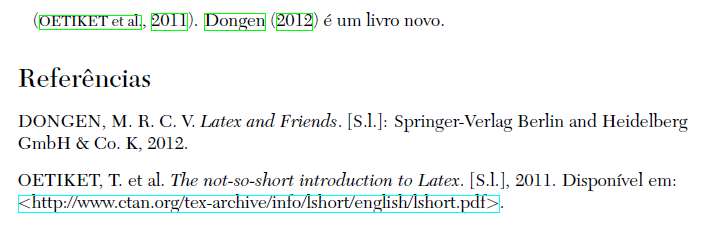
\includegraphics[width=0.7\linewidth]{./abntex-bibliografia-figura}
\caption{Exemplo de bibliografia gerada com abntex.}
\label{fig:abntex-bibliografia-figura}
\end{figure}

Código da figura \ref{fig:abntex-bibliografia-figura}:

\begin{verbatim}
\usepackage[alf]{abntex2cite}

\begin{document}
\cite{lshort}.
\citeonline{dongen_latex_2012} é um livro novo.

%\nocite{*} % --> não use esse comando com abntex2cite
\bibliography{latex}

\end{document}
\end{verbatim}


\begin{figure}
\centering
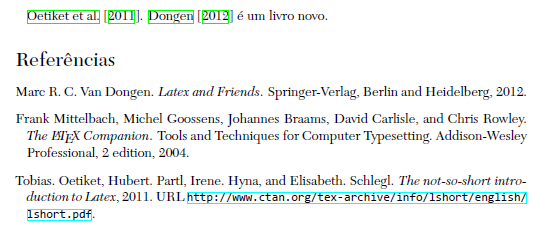
\includegraphics[width=0.7\linewidth]{./natbib-test-plainnat}
\caption{\texttt{natbib} e estilo \texttt{plainnat}.}
\label{fig:natbib-test-plainnat}
\end{figure}

Código da figura \ref{fig:natbib-test-plainnat}:

\begin{verbatim}
\usepackage{natbib}

\begin{document}
\cite{lshort}.
\citet{dongen_latex_2012} é um livro novo.

\nocite{*}
\bibliography{latex}
\bibliographystyle{plainnat}

\end{document}
\end{verbatim}



Para serem processadas as referências e a bibliografia, deve-se compilar o documento mais que uma vez:

\begin{enumerate}
\item xelatex ``arquivo" \item 
bibtex ``arquivo" \item
xelatex ``arquivo" \item 
xelatex ``arquivo" 
\end{enumerate}


Na primeira compilação, aparecerão ``erros'' como:

\begin{verbatim}
LaTeX Warning: Citation `lamport94' on page 1 undefined on input line 21.
...
LaTeX Warning: There were undefined references.
\end{verbatim}


Na segunda, pode aparecer a mensagem: \texttt{``LaTeX Warning: Label(s) may have changed. Rerun to get cross-references right."} As referências no arquivo final ainda estão indefinidas ou mal definidas, com [??] ao invés da referência. Ao compilar mais uma vez, esses erros desaparecerão.

Além do \texttt{bibtex}, também é possível utilizar o \texttt{biblatex}, cuja vantagem é a inserção de caracteres acentuados ou utf8:

\begin{figure}
\centering
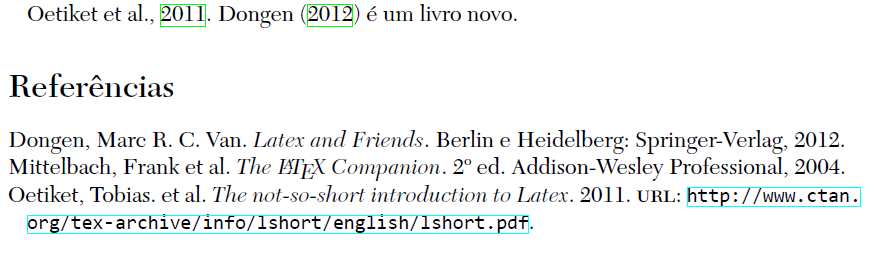
\includegraphics[width=0.7\linewidth]{./biblatex-figura}
\caption{Exemplo de bibliografia gerada com \texttt{biblatex}.}
\label{fig:biblatex-figura}
\end{figure}

Código da figura \ref{fig:biblatex-figura}:

\begin{verbatim}
\usepackage[style=historian,citestyle=authoryear,natbib=true,doi=false,backend=bibtex]{biblatex}
\usepackage{csquotes}
\DefineBibliographyStrings{brazil}{namedash={---------}}
\addbibresource{latex} %substitui o \bibliography{xxx} do bibtex

\begin{document}
\cite{lshort}.
\citet{dongen_latex_2012} é um livro novo.

\nocite{*}

\printbibliography %para gerar bibliografia

\end{document}

\end{verbatim}




\chapter{Tabelas}
É fácil criar tabelas simples em \LaTeX, mas tabelas mais complicadas podem ser difíceis. Mas você pode converter as tabelas do Excel ou OpenOffice com plugins:
\url{ http://calc2latex.sourceforge.net/} para OpenOffice/Libreoffice e \url{http://www.ctan.org/tex-archive/support/excel2latex/} para Excel. 

Há dois ambientes usados em tabelas: \texttt{tabular} e \texttt{table}. Geralmente têm a seguinte forma:

\begin{table}[h!]
\centering
\caption{Exemplo de tabela}
\label{exemplotabela}
\begin{tabular}{llp{3cm}}
\hline
texto & texto & texto\\
\hline
texto & texto & texto\\
\hline
\end{tabular}
\end{table}

que foi criada com o seguinte código:

\begin{verbatim}
\begin{table}[h!]
\centering
\caption{Título da tabela}
\label{exemplotabela}
\begin{tabular}{llp{3cm}}
\hline
texto & texto & texto\\
\hline
texto & texto & texto\\
\hline
\end{tabular}
\end{table}
\end{verbatim}

O especificador \verb+[h!]+ obriga a colocar a tabela exatamente ``aqui" (h=here). Ela também pode ficar em baixo, no fim da página (\texttt{b}=bottom) ou no centro (\texttt{c}) da página. Se você não explicitar, o \LaTeX fará um cálculo para inserir a tabela onde ficar melhor, tipograficamente. O acento de exclamação serve para passar por cima dos cálculos e colocar a tabela \textit{exatamente} onde você quer. Os comandos utilizados para 
tabelas encontram-se na página \pageref{comandosdetabelas}.

\begin{table}
\centering
\caption{Comandos utilizados para tabelas}
\label{comandosdetabelas}
\begin{tabular}{lp{8cm}}
\toprule
& \\
l & coluna justificada à esquerda\\
c & coluna centralizada\\
r & coluna justificada à direita\\
\verb+p{largura}+ &coluna com texto alinhado no topo, com largura especificada (em centímetros ou outra medida)\\
\verb+m{largura}+ & o mesmo acima, mas alinhado no meio da célula (requer pacote \texttt{array})\\
 \verb+m{largura}+ & o mesmo acima, mas alinhado no fim da célula (requer pacote \texttt{array})\\
 | & linha vertical\\
 || & duas linhas verticais\\
 \verb+\hline+ & linha horizontal\\
 \& & separador de colunas\\
\textbackslash \textbackslash & começa nova linha (espaço adicional pode ser especificado usando colchetes: por exemplo, \verb+[6pt]+ especifica um espaço de 6 pontos depois da linha)\\
 \verb+\newline+ & começa nova linha dentro da mesma célula\\
 \verb+\cline{i-j}+ & linha parcial horizontal começando na coluna \textit{i} e terminando na coluna \textit{j}.\\
 \bottomrule
\end{tabular}
\end{table}


\section{Tabelas longas}
Para tabelas muito longas (de mais de uma página), podemos usar o ambiente/pacote \texttt{longtable}, ao invés de \texttt{table}:\footnote{Notas de rodapé funcionam com \texttt{longtable}, mas não com \texttt{table}.}

\begin{verbatim}
\begin{longtable}{opções}
....
\end{longtable}
\end{verbatim}

Se você preferir girar a tabela na vertical, use o pacote \texttt{rotating} e o ambiente \texttt{sidewaystable}:

\begin{verbatim}
\usepackage{rotating}

\begin{sidewaystable}
   \begin{tabular}...
   \end{tabular}
\end{sidewaystable}
\end{verbatim}

Finalmente, você poder usar o comando \verb+\listoftables+ para gerar uma lista de tabelas (no começo do texto)

Para exemplos mais elaborados (e que dificilmente você utilizará), ver \url{http://en.wikibooks.org/wiki/LaTeX/Tables}


\chapter{Formatação}

``Formatação" se refere à maioria das coisas que se pode fazer para mudar a aparência do texto: estilo do texto, fonte, tamanho; alinhamento de parágrafos, espaço entre as linhas, indentação, tipos especiais de parágrafo, notas de rodapé, notas de margem etc.

Muitas dessas formatações são exigidas para diferenciar certos elementos do resto do texto. Frequentemente precisamos de enfatizar palavras ou frases. Notas de rodapé são úteis para fornecer informação e explicação extra sem interromper o fluxo do texto principal. Portanto, a formatação é muito importante. No entanto, também é muito fácil abusar dela, e um documento excessivamente rebuscado pode ter uma aparência pior e ser menos legível do que um sem qualquer formatação.

\section{Listas}

A formatação conveniente e predizível de listas é uma das muitas vantagens de usar \LaTeX. Muitos usuários de processadores de texto ficam frequentemente frustrados pelas tentativas desajeitadas do software de perceber quando o usuário quer que as listas comecem e terminem. Por outro lado, \LaTeX{} lhe dá muito mais estabilidade na geração de listas.

Há basicamente três tipos de listas: itens, enumeração e descrição.

\subsection{Itemizar}


\begin{tabular}{ll}
\begin{minipage}{.5\textwidth}
\begin{verbatim}
\begin{itemize}
\item O primeiro item 
\item O segundo item 
\item O terceiro item.
\end{itemize}
\end{verbatim}
\end{minipage}
&
\begin{minipage}{.5\textwidth}
\begin{itemize}
\item O primeiro item 
\item O segundo item 
\item O terceiro item.
\end{itemize}\end{minipage}\\
\end{tabular}


\subsection{Enumeração}

\begin{tabular}{ll}
\begin{minipage}{.5\textwidth}
\begin{verbatim}
\begin{enumerate}
\item O primeiro item 
\item O segundo item 
\item O terceiro item.
\end{enumerate}
\end{verbatim}
\end{minipage}
&
\begin{minipage}{.5\textwidth}
\begin{enumerate}
\item O primeiro item 
\item O segundo item 
\item O terceiro item.
\end{enumerate}\end{minipage}\\
\end{tabular}

\subsection{Descrição}

\begin{tabular}{ll}
\begin{minipage}{.5\textwidth}
\begin{verbatim}
\begin{description}
\item O primeiro item 
\item O segundo item 
\item O terceiro item.
\end{description}
\end{verbatim}
\end{minipage}
&
\begin{minipage}{.5\textwidth}
\begin{description}
\item[Objeto] Descrição do primeiro item 
\item[Objeto] Descrição do segundo item 
\item[Objeto] Descrição do terceiro item.
\end{description}\end{minipage}\\
\end{tabular}


\subsection{Listas aninhadas (listas dentro de listas)}

\begin{tabular}{ll}
\begin{minipage}{.5\textwidth}
\begin{verbatim}
\begin{enumerate}
   \item O primeiro item
   \begin{enumerate}
     \item Primeiro subitem
     \item Segundo subitem
   \end{enumerate}
   \item O segundo item
   \item O terceiro item
\end{enumerate}
\end{verbatim}
\end{minipage}
&
\begin{minipage}{.5\textwidth}
\begin{enumerate}
   \item O primeiro item
   \begin{enumerate}
     \item Primeiro subitem
     \item Segundo subitem
   \end{enumerate}
   \item O segundo item
   \item O terceiro item
\end{enumerate}
\end{minipage}\\
\end{tabular}

\bigskip


Você pode personalizar as listas com o pacote \texttt{enumitem}.\label{enumitem} Assim, para listas como 1.1, 1.2, 1.3:
\medskip

\begin{tabular}{ll}
\begin{minipage}{.5\textwidth}
\begin{verbatim}
\begin{enumerate}
  \item O primeiro item
  \begin{enumerate}[label*=\arabic*.]
     \item Primeiro subitem
     \item Segundo subitem
    \begin{enumerate}[label*=\arabic*.]
      \item Primeiro sub-subitem
      \item Segundo sub-subitem
    \end{enumerate}
  \end{enumerate}
\end{enumerate}
\end{verbatim}
\end{minipage}
&
\begin{minipage}{.5\textwidth}
\begin{enumerate}
  \item O primeiro item
  \begin{enumerate}[label*=\arabic*.]
     \item Primeiro subitem
     \item Segundo subitem
    \begin{enumerate}[label*=\arabic*.]
      \item Primeiro sub-subitem
      \item Segundo sub-subitem
    \end{enumerate}
  \end{enumerate}
\end{enumerate}
\end{minipage}\\
\end{tabular}

\bigskip

Mas se você só vai usar esse tipo de listas no seu documento, é mais fácil redefinir os comandos:

\begin{verbatim}
\renewcommand{\labelenumi}{\arabic{enumi}.} 
\renewcommand{\labelenumii}{\arabic{enumi}.\arabic{enumii}}
\end{verbatim}

Você também pode especificar o tipo de contador que quer: numerais romanos, em maiúsculas, minúsculas ou itálicos. Por exemplo:

\bigskip

\begin{tabular}{ll}
\begin{minipage}{.5\textwidth}
\begin{verbatim}
\begin{enumerate}[label=\Roman*]
\item Primeiro
\item Segundo
\item Terceiro
\end{enumerate}
\end{verbatim}
\end{minipage}
&
\begin{minipage}{.5\textwidth}
\begin{enumerate}
\begin{enumerate}[label=\Roman*]
\item Primeiro
\item Segundo
\item Terceiro
\end{enumerate}
\end{enumerate}
\end{minipage}\\
\end{tabular}

\bigskip

As outras opções do pacote enumitem (para \verb+\begin{enumerate}[opções]+) são: 

\begin{tabular}{ccccc}
\verb+\Alph*+ & \verb+\alph*+ & \verb+\Roman*+ & \verb+\roman*+ & \verb+\arabic*+\\
\end{tabular}

Para soluções mais simples, o pacote \verb+enumerate+ é mais intuitivo:

\begin{verbatim}
\begin{enumerate}[a)]
\item \item \item 
\end{enumerate}
\end{verbatim}

\begin{enumerate}[label=\alph*)]
\item \item \item 
\end{enumerate}

\begin{verbatim}
\begin{enumerate}[I.]
\item item item 
\end{enumerate}
\end{verbatim}

\begin{enumerate}[label=\Roman*.]
\item \item \item 
\end{enumerate}

No entanto, é bom ter cuidado para só usar \textit{um} dos dois pacotes (\texttt{enumerate} ou \texttt{enumitem}).

\subsection{Listas em múltiplas colunas}

Usando o pacote \texttt{multicol} --- \verb+\usepackage{multicol}+---, podemos colocar listas em várias colunas:

\bigskip

\begin{verbatim}
\begin{multicols}{2}
\begin{enumerate}
    \item a
    \item b
    \item c
    \item d
    \item e
    \item f
\end{enumerate}
\end{multicols}
\end{document}
\end{verbatim}

\begin{multicols}{2}
\begin{enumerate}
    \item a
    \item b
    \item c
    \item d
    \item e
    \item f
\end{enumerate}
\end{multicols}




\section{Hifenização}
O \LaTeX{} hifenizará as palavras sempre que necessário. Se houver uma palavra que ele não souber hifenizar, e se ela precisar de hifenização, ela sairá da margem da página no documento final.

Para remediar essa situação, você pode fazer uma lista de hifenizações no começo do seu documento:

\begin{verbatim}
\hyphenation{lista de palavras}
\end{verbatim}

E adicionar as palavras separadas com um hífen.

Uma outra solução é simplesmente hifenizar a palavra recalcitrante com \verb+\-+:

\begin{verbatim}
in\-cons\-ti\-tu\-ci\-o\-na\-lis\-si\-ma\-men\-te
\end{verbatim}

Se você quiser que uma palavra não seja hifenizada, use o comando \verb+\mbox{texto}+, que fará com que a palavra fique sempre junta na mesma linha.

O comando \verb+\fbox{texto}+ é semelhante a \verb+\mbox{}+, mas desenha uma \fbox{caixa} ao redor do texto.

\section{Aspas}
O \LaTeX{} trata aspas da esquerda e da direita como entidades diferentes. Para abrir aspas, escreva a crase (\verb+`+) ou (\verb+``+), e, para fechar, feche com um ou dois apóstrofos (\verb+'+ ou \verb+''+) ou simplesmente as aspas normais do seu teclado (\verb+"+).

Exemplos:

\begin{table}[htbp]
\caption{Aspas}
\label{aspas}
\begin{tabular}{lp{7cm}}
\verb+ `Citar' em Latex+	& `Citar' em Latex\\

\verb+ ``Citar'' em Latex+	& ``Citar'' em Latex\\


\verb+ ``quote" in Latex+	& ``Citar" em Latex\\


\verb+ ,,quote'' in Latex+	& ,,citar'' em Latex\\


\verb+ ``Please press the `x' key.''+	& ``Por favor, pressione a tecla `x'."\\

\verb+<<Guillemets>>+ & \textfrench{<< Guillemets >>} (aspas angulares, utilizadas no português europeu, em francês e alemão, entre outras)\\


\end{tabular}
\end{table}

Geralmente os programas de edição em \LaTeX{} como TexStudio e TexWorks têm a opção de mudar as aspas automaticamente, então você geralmente não precisa de se preocupar com isso. Procure no menu de opções do programa.

Para usar estilos de apóstrofes europeus (se não estiver usando o compilador \texttt{xelatex}), precisamos de colocar no preâmbulo:

\begin{verbatim}
\usepackage[T1]{fontenc}
\end{verbatim}





\section{Travessão, hífen, meia-risca}

Um travessão (---) em \LaTeX{} é inserido com: \verb+---+.

Um hífen (utilizados para ligar palavras compostas e separar sílabas) é inserido com o hífen normal do teclado.

Uma meia-risca\footnote{A meia-risca (também chamada de traço de ligação, meio-traço ou traço médio) é um sinal de pontuação que serve para unir os valores extremos de uma série, como números (1–10), letras (A–Z) ou outras, indicando ausência de intervalos na enumeração. Serve igualmente para unir palavras que tenham um nexo lógico (ex.: a viagem Lisboa–Porto). [\ldots] A meia-risca não é o mesmo que o hífen nem que o travessão. (Fonte: \url{http://pt.wikipedia.org/wiki/Meia-risca}.)} (--) é inserida com \verb+--+.


\section{Espaço entre palavras e frases}
O \LaTeX{} calcula (muito bem, melhor que programas como Word e OpenOffice) os espaços entre as palavras para margens justificadas. Mas ele também coloca um pequeno espaço adicional entre as frases, o que não é muito usual hoje em dia. Para colocar um espaço normal entre as frases, é só adicionar

\begin{verbatim}
\frenchspacing
\end{verbatim}

depois de \verb+\begin{document}+.

Para colocar espaços adicionais entre parágrafos, podem-se usar os seguintes comandos:

\begin{verbatim}
\medskip
\end{verbatim}

\begin{verbatim}
\bigskip
\end{verbatim}

Ou especificar em centímetros/pontos:

\begin{verbatim}
\\[10cm]
\end{verbatim}


\section{Enfatizando texto}
Para enfatizar uma palavra ou frase, usamos o comando \verb+\emph+:

\begin{tabular}{ll}
\verb+\emph{Enfatizar} uma palavra+ & \emph{Enfatizar} uma palavra\\
\end{tabular}

Isso também pode ser feito com os comandos \verb+\textit{}+ (``texto em itálico") e, para negrito, \verb+\textbf{}+.

\section{Estilos de fonte}
Os estilos de fonte e seus comandos são explicados na tabela \ref{estilosdefonte}.


\begin{table*}
\caption{Estilos de fonte}
\label{estilosdefonte}
\centering
\begin{tabular}{lll}
\toprule
\textbf{Comando \LaTeX{}} & \textbf{Equivalente a} & \textbf{Resultado}\\
\midrule
\verb+\textnormal{}+ & \verb+{\normalfont ... }+ & a fonte normal do documento\\
\verb+\emph{...}+ & \verb+{\em}+ & \textit{ênfase} (geralmente itálico)\\
\verb+\textrm{...}+ & \verb+{\rmfamily}+ & fonte romana/serifada\\
\verb+\textsf{...}+ & \verb+{\sffamily}+ & {\fontspec{Myriad Pro}fonte sem serifas}\\
\verb+\texttt{...}+ & \verb+{\ttfamily}+ & \texttt{fonte com largura fixa (monoespaçada)}\\
\verb+\textit{...}+ & \verb+{\itshape}+ & \textit{itálico}\\
\verb+\textbf{...}+ & \verb+{\bfseries}+ & \textbf{negrito}\\
\verb+\textsc{...}+ & \verb+{\scshape}+ & \textsc{Versalete (Small Capitals)}\\
\bottomrule
\end{tabular}
\end{table*}

O sublinhado pode ser feito com \verb+\underline{...}+, mas as palavras com sublinhado não se separam corretamente. Para resolver esse problema, insira \newline\verb+\usepackage[normalem]{ulem}+ no preâmbulo. Com o pacote \texttt{ulem}, você pode usar estes comandos: \verb+\uline{}+ (\uline{sublinhado}) para ênfase; \verb+\uwave{}+ para \uwave{ondulado} e \verb+\sout{...}+ para \sout{cortado}.\footnote{Você pode estar se perguntando: por que essa complicação para sublinhado? A resposta é simples: o sublinhado (assim como o negrito) não é uma prática tipográfica comum. Abra um livro e veja se há algum sublinhado ou negrito. O sublinhado (assim como outras coisas) era usado para ênfase em máquinas de datilografar, e passou para algumas regras de redação acadêmica por isso.
}
1
Um ambiente útil para gerar o texto exatamente como foi digitado (como códigos), é o ambiente \texttt{verbatim}:

\begin{center}
\verb+\begin{verbatim}+
...
\verb+\end{verbatim}+
\end{center}

Tudo o que for posto dentro desse ambiente aparecerá no texto final em fonte monoespaçada exatamente como está. Para pouco texto, podemos usar o comando 

\begin{verbatim}
\verb+coloque seu texto/comando aqui, entre os ++ ...+
\end{verbatim}

\section{Tamanho de fonte}
Há alguns comandos predefinidos para tamanhos de fonte. Na verdade, raramente você vai se preocupar com questões como: Qual o tamanho do título? Qual o tamanho do título da seção? Qual o espaço depois do título e antes do texto? Mas se você quiser fazer alguma coisa manualmente, os comandos da tabela \ref{tamanhodotexto} são úteis.

\begin{table}
\caption{Tamanho do texto}
\label{tamanhodotexto}
\centering
\begin{tabular}{lc}
&\\
\verb+\tiny+ & {\tiny exemplo de texto}\\
\verb+\scriptsize+ & {\scriptsize exemplo de texto}\\
\verb+\footnotesize+ & {\footnotesize exemplo de texto}\\
\verb+\small+ & {\small exemplo de texto}\\
\verb+\normalsize+ & {\normalsize exemplo de texto}\\
\verb+\large+ & {\large exemplo de texto}\\
\verb+\Large+ & {\Large exemplo de texto}\\
\verb+\LARGE+ & {\LARGE exemplo de texto}\\
\verb+\huge+ & {\huge exemplo de texto}\\
\verb+\Huge+ & {\Huge exemplo de texto}\\
\end{tabular}
\end{table}

Esses comandos afetam \textit{todo} o texto que vai depois deles, então se quiser limitar a uma parte do texto, coloque entre chaves. Exemplo:

\begin{tabular}{ll}
\verb+{\large exemplo de texto}+ & {\large exemplo de texto}
\end{tabular}

\section{Sobrescrito e subscrito}
Para sobrescrito (\textsuperscript{o,a,1,2,3}), usamos: \verb+\textsuperscript{}+

Para subscrito (\textsubscript{o,a,1,2,3}), usamos: \verb+\texsubscript{}+ (com o pacote \texttt{fixltx2e}).

Para escrever fórmulas químicas, é útil o pacote \texttt{mhchem} (\url{http://www.ctan.org/tex-archive/macros/latex/contrib/mhchem/}). Coloque no preâmbulo:

\begin{verbatim}
\usepackage[version=3]{mhchem}
\end{verbatim}

E escreva suas fórmulas:

\begin{tabular}{ll}
\verb+Sulfato de amônio é \ce{(NH4)2SO4}.+ & Sulfato de amônio é \ce{(NH4)2SO4}.\\
\end{tabular}

\section{Símbolos}
O \LaTeX{} fornece uma imensa quantidade de símbolos, matemáticos ou não. Se você estiver usando um editor de textos como o TexStudio ou Texmaker, você não precisa decorar os comandos, é simplesmente apontar e clicar. Mas alguns pacotes têm que ser colocados no preâmbulo. Os pacotes:

\begin{verbatim}
\usepackage{textcomp}
\usepackage[official]{eurosym}
\usepackage{amssymb}
\usepackage{wasysym}
\end{verbatim}

Vão suprir quase todas as suas necessidades (tabela \ref{simbolos}).

\begin{table}
\caption{Símbolos comuns}
\label{simbolos}
\centering
\begin{tabular}{lc}
&\\
\verb+\textdollar+ & \textdollar\\
\verb+\pounds+ & \pounds\\
\verb+\textordmasculine+ & \textordmasculine\\
\verb+\textordfeminine+ & \textordfeminine\\
\verb+\dag+ & \dag \\
\verb+\ddag+ & \ddag \\
\verb+\S+ & \S \\
\verb+\P+ & \P \\
\verb+\textregistered+ & \textregistered \\
\verb+\officialeuro+ & \officialeuro \\
\verb+\textcopyright+ & \textcopyright \\
\verb+\male+ & \male \\
\verb+\female+ & \female \\
\end{tabular}
\end{table}


\begin{table}
\caption{Signos astrológicos e do zodíaco}
\label{signos}
\centering
\begin{tabular}{cccc}
\toprule
&&&\\
\verb+\vernal+ & \vernal & \verb+\ascnode+ & \ascnode\\
\verb+\descnode+ & \descnode & \verb+\fullmoon+ & \fullmoon\\
\verb+\newmoon+ & \newmoon&
\verb+\leftmoon+ & \leftmoon\\
\verb+\rightmoon+ & \rightmoon&
\verb+\astrosun+ & \astrosun \\
\verb+\mercury+ & \mercury&
\verb+\venus+ & \venus\\
\verb+\earth+ & \earth&
\verb+\mars+ & \mars\\
\verb+\jupiter+ & \jupiter&
\verb+\saturn+ & \saturn\\
\verb+\uranus+ & \uranus&
\verb+\neptune+ & \neptune\\
\verb+\pluto+ & \pluto&
\verb+\aries+ & \aries\\
\verb+\taurus+ & \taurus&
\verb+\gemini+ & \gemini\\
\verb+\cancer+ & \cancer&
\verb+\leo+ & \leo\\
\verb+\virgo+ & \virgo&
\verb+\libra+ & \libra\\
\verb+\scorpio+ & \scorpio&
\verb+\sagittarius+ & \sagittarius\\
\verb+\capricornus+ & \capricornus&
\verb+\aquarius+ & \aquarius\\
\verb+\pisces+ & \pisces & & \\
\bottomrule
\end{tabular}
\end{table}

\section{Formatação de parágrafos}
Os parágrafos em \LaTeX{} são geralmente justificados, mas se quiser em outro estilo, pode usar os ambientes/comandos:

\begin{table}
\caption{Alinhamento de parágrafos}
\label{paragrafos}
\centering
\begin{tabular}{lll}
\toprule
\textbf{Alinhamento} & \textbf{Ambiente} & \textbf{Comando}\\
\midrule
Justificado à esquerda & flushleft & \verb+\raggedright+\\
Justificado à direita & flushright & \verb+\raggedleft+\\
Centro & center & \verb+\centering+\\

\bottomrule
\end{tabular}
\end{table}

Exemplo:

\begin{verbatim}
\begin{center}
Este é um texto centralizado.
\end{center}
\end{verbatim}

\medskip

\begin{center}
Este é um texto centralizado.
\end{center}

Os parágrafos são indentados (distância entre a margem e a primeira linha do parágrafo) automaticamente. Você pode definir a indentação com o comando:

\begin{verbatim}
\setlength{\parindent}{1cm}
\end{verbatim}

substituindo o número em cm.

Para mudar o espaçamento entrelinhas, use o pacote \verb+\usepackage{setspace}+. Esse pacote fornece os ambientes:

\begin{verbatim}
\begin{doublespace}
...
\end{doublespace}

\begin{onehalfspace}
...
\end{onehalfspace}

\begin{singlespace}
...
\end{singlespace}
\end{verbatim}

E os comandos:

\begin{verbatim}
\doublespacing

\onehalfspacing

\singlespacing

\end{verbatim}

Para espaço duplo, um e meio, e um, respectivamente.

\section{Inserção de hiperlinks}
Para inserir links que podem ser abertos diretamente no seu navegador ao clicar no pdf, use o pacote

\begin{verbatim}
\usepackage{hyperref}
\end{verbatim}

ou 

\begin{verbatim}
\usepackage{url}
\end{verbatim}

e insira o link no comando. Por exemplo:

\begin{minipage}{.5\textwidth}
\begin{verbatim}
\url{www.wikipedia.org}
\end{verbatim}
\end{minipage}

\begin{minipage}{.5\textwidth}
\url{www.wikipedia.org}
\end{minipage}

O pacote \texttt{hyperref} deve ser colocado como último entre os pacotes do preâmbulo, para evitar incompatibilidades.

Para inserir e-mails clicáveis a partir do pdf, siga este procedimento:

\begin{verbatim}
\href{mailto:meuemail@wikibooks.org}{meuemail@wikibooks.org}
\end{verbatim}

\href{mailto:meuemail@wikibooks.org}{meuemail@wikibooks.org}




\section{Citando textos}
Os ambientes para citação são:

\begin{description}
\item[quote] para uma citação de geralmente não mais que um parágrafo (parágrafos são separados por linha em branco)
\item[quotation] citações longas, geralmente de mais de um parágrafo (parágrafos são indentados)
\item[verse] para poesia. Novas linhas com o comando \textbackslash\textbackslash, e novas estrofes, com uma linha em branco (dois \textsf{ENTER}).
\item[citacao] comando do pacote \texttt{abntex2} para citações segundo as regras da ABNT.
\end{description}

\section{Notas de rodapé}
São inseridas com o comando: \verb+\footnote{...}+.

\section{Cabeçalhos}
Há duas maneiras ``fáceis'' de inserir cabeçalhos, quando necessário: o pacote \texttt{fancyhdr} e o pacote \texttt{scrpage2} (do pacote KOMA-Script{}). De qualquer forma, as classes \texttt{book} e \texttt{scrbook} inserem automaticamente os cabeçalhos, com o número no rodapé.

Se você quiser inserir o número do lado direito no começo da página (uma prática usual por aqui), o jeito mais fácil é pôr \verb+\pagestyle{myheadings}+ depois de \verb+\begin{document}+ e \verb+\thispagestyle{myheadings}+ depois do começo de cada capítulo. %O pacote \texttt{abntex2} já faz tudo isso automaticamente.

\section{Modo matemático}
O \LaTeX{} é geralmente usado por matemáticos ou físicos ou pesquisadores que precisam de muitos símbolos e fórmulas. Mas podemos usar simplesmente porque ele permite um resultado superior sem muito esforço --- seja com puro texto, com muitas fórmulas ou muitas figuras. O público-alvo deste ``manual'' não é esse tipo de usuário, por um simples motivo: o redator (leia-se: eu) não é matemático, não usa fórmulas. Se você precisa de trabalhar com matemática, sugiro dar uma olhada em: \url{http://en.wikibooks.org/wiki/LaTeX/Mathematics} e/ou \url{http://mirrors.ctan.org/info/lshort/portuguese-BR/lshortBR.pdf}.


\chapter{Figuras}

\section{Incluindo imagens}
Para incluir imagens, usamos o pacote \texttt{graphicx} (\verb+\usepackage{graphicx}+ no preâmbulo). 
Além das imagens de formato comum (.jpeg, .png), podem ser incluídas imagens em pdf.

O comando para incluir imagens é:

\begin{verbatim}
\includegraphics[opções]{nome do arquivo}
\end{verbatim}

As opções para inserir imagens são:

\begin{description}
\item[width=xx] Largura=xx. Ex.: \texttt{width=5cm}
\item[height=xx] Altura=xx. Ex.: \texttt{height=10cm}
\item[scale=xx] Escala no fator=xx; por exemplo: \texttt{scale=0.5} reduz o tamanho da imagem pela metade, \texttt{scale=2} aumenta duas vezes.
\item[angle=xx] Roda a imagem em xx graus (sentido anti-horário).
\item[page=x] Se o arquivo de imagem for um pdf com mais de uma página, esse parâmetro possibilita escolher uma outra página que não a primeira.
\end{description} 

Para usar mais de uma opção ao mesmo tempo, separe com uma vírgula. A ordem dos comandos pode importar: você deve rodar a imagem (com um ângulo) e \textit{depois} especificar a largura.

\begin{figure}
\centering
\includegraphics[width=.8\textwidth]{femmevaguecourbet}
\caption[Gustave Courbet, \textit{Femme à la Vague} (1868). ]{Gustave Courbet, \textit{Femme à la Vague}, óleo sobre tela, 1868. Metropolitan Museum of Art.}
\label{courbet}
\end{figure}



\section{Onde guardar as imagens do seu texto}

O mais fácil e prático é guardar os arquivos de imagem na mesma pasta do arquivo .tex. Se você quiser que o LaTeX procure as imagens em outro lugar, você deve indicar onde elas se encontram com o comando, por exemplo:


\begin{verbatim}
\graphicspath{~/Pictures} %(geralmente é o diretório de imagens para Linux e Mac)
\graphicspath{{c:/mypict~1/}} %(geralmente no Windows: My Pictures)
\end{verbatim}

Mas você deve ter em mente: não use espaços ou acentos no nome dos arquivos ou das pastas.


\section{Exemplos}

\begin{verbatim}
\includegraphics{coroavray}
\end{verbatim}

Essa imagem, no entanto, é grande demais e ultrapassa o tamanho da página (por isso nem a exibimos aqui). Se quisermos diminuir o seu tamanho, podemos especificar a escala, a largura e a altura. Assim:


\begin{verbatim}
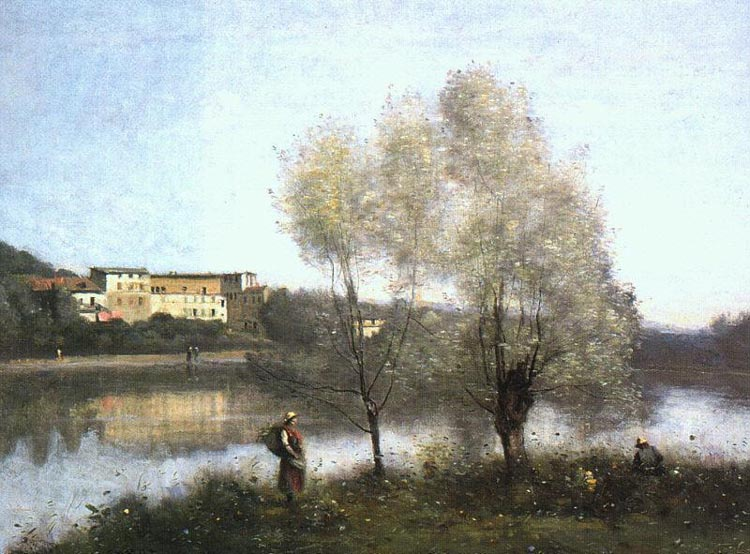
\includegraphics[scale=.5]{corotavray}
\end{verbatim}

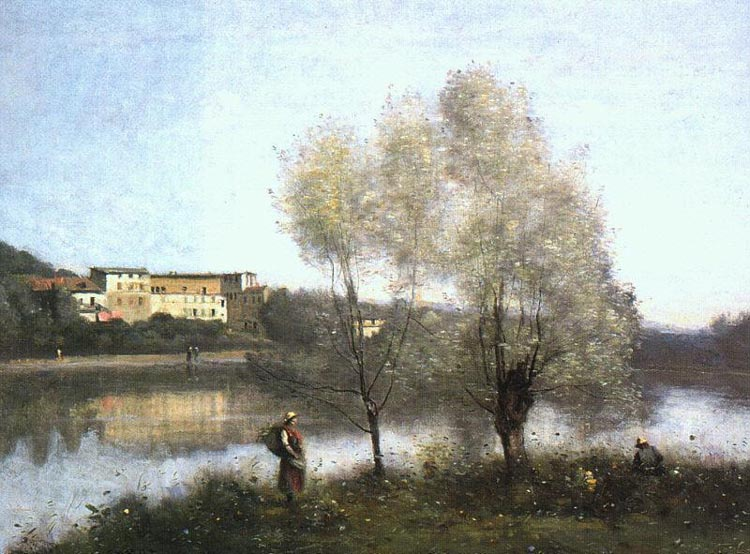
\includegraphics[scale=.5]{corotavray}

\medskip

\begin{verbatim}
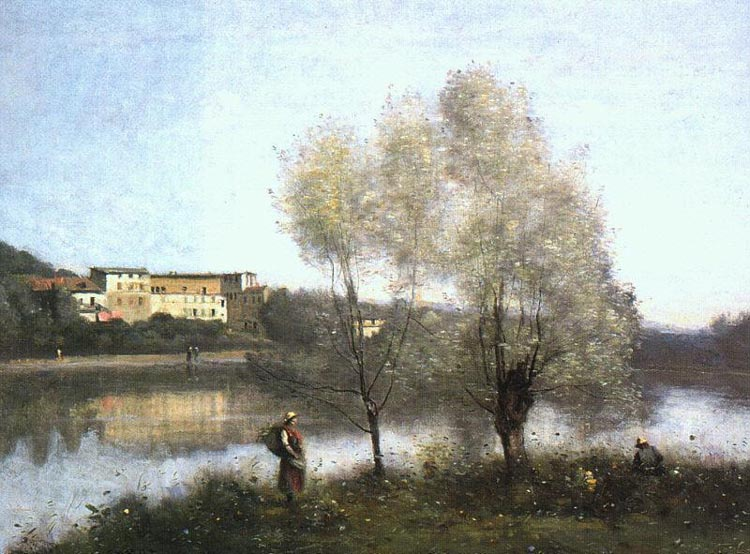
\includegraphics[height=10cm]{corotavray}
\end{verbatim}


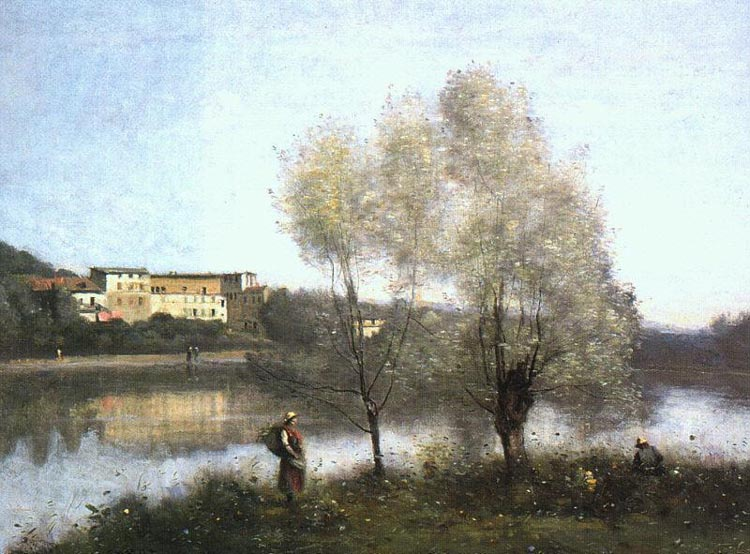
\includegraphics[height=10cm]{corotavray}

\medskip

\begin{verbatim}
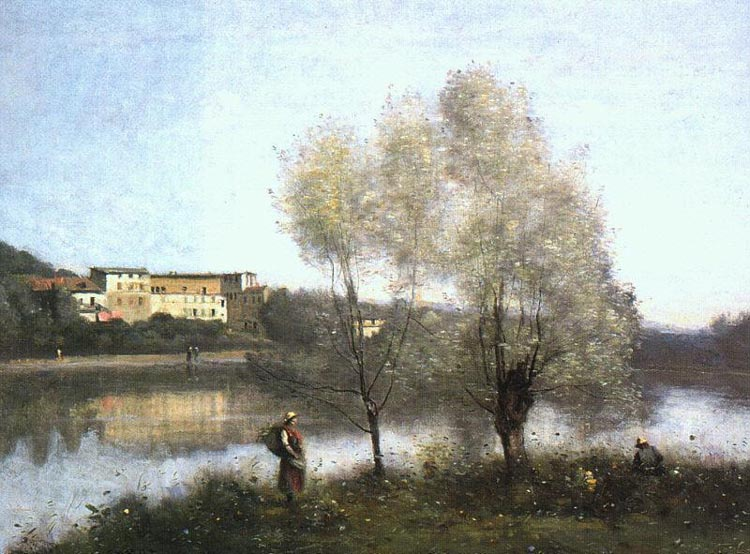
\includegraphics[width=.8\textwidth]{corotavray}
\end{verbatim}

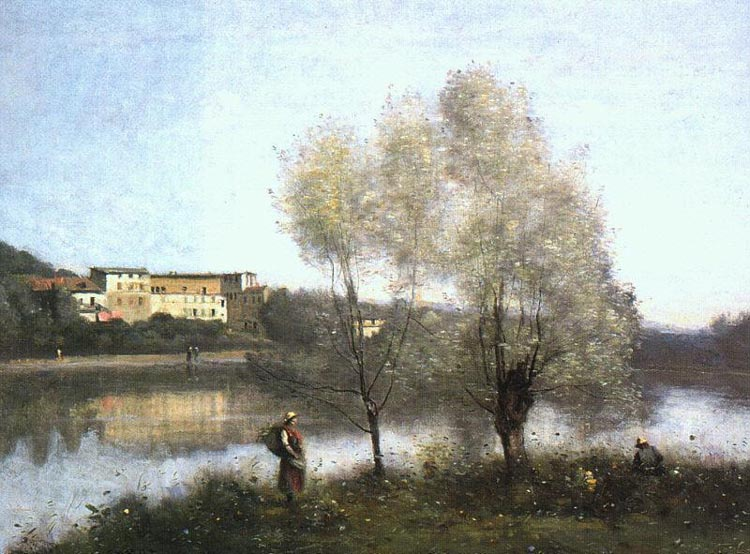
\includegraphics[width=.8\textwidth]{corotavray}

\medskip

Neste último caso, especificamos a largura em relação ao texto da página (\verb+\textwidth+, que poderia ser também a linha, no caso de textos com colunas: \verb+\linewidth+ ou toda a altura do texto: \verb+\textheight+). 

Essa maneira de inserir imagens é prática porque assim você não precisa de ficar se preocupando com medidas.

\section{Imagens como figuras}
Há ocasiões em que você pode querer que sua imagem tenha uma legenda e talvez uma referência cruzada. Isso é feito usando o ambiente \texttt{figure}. O código mínimo para criar uma figura é:

\begin{verbatim}
\begin{figure}[opções]
\includegraphics{imagem}
\end{figure}
\end{verbatim}

O programa vai calcular onde será melhor colocar a figura para não interromper o fluxo do texto. As opções [] acima podem ser [h], para (aproximadamente) \textit{aqui} (``here''); t, para por a figura no topo da página; b, no fim da página ( ``bottom''); p, para uma página especial com figuras. Para forçar o programa a colocar exatamente onde você quer, use a exclamação, por exemplo, [h!], ``exatamente aqui''.

Você pode usar o comando \verb+\listoffigures+ para criar uma lista de figuras (no começo do texto)


O exemplo anterior é bem simples e não tem muitas funções. 
Geralmente queremos algo como na figura \ref{corot}, criado com o seguinte código:

\begin{verbatim}
\begin{figure}[h]
\caption[\textit{Ville d'Avray} de Corot (ca. 1867).]{Jean-Baptiste Corot. 
\textit{Ville d'Avray} (ca. 1867).
Fonte: Wikipedia 
(\url{http://fr.wikipedia.org/wiki/Fichier:Corot.villedavray.750pix.jpg})}
\label{corot}
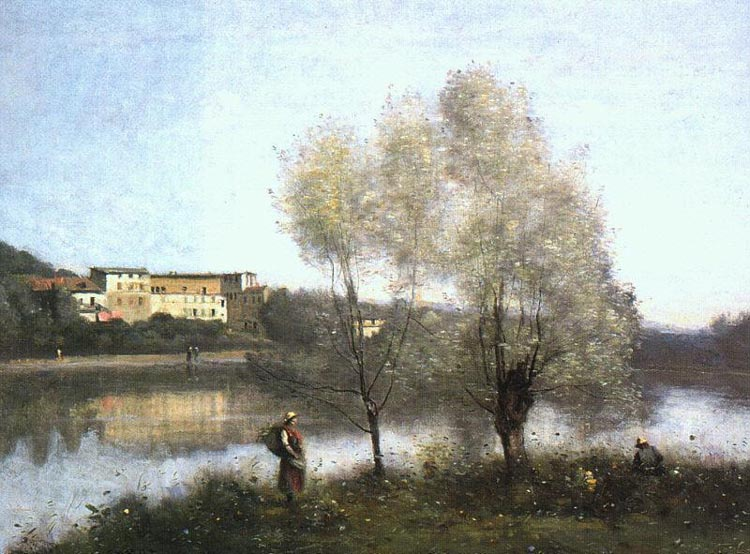
\includegraphics[width=.8\textwidth]{corotavray}
\end{figure}
\end{verbatim}

\begin{figure}[htpb]
\centering
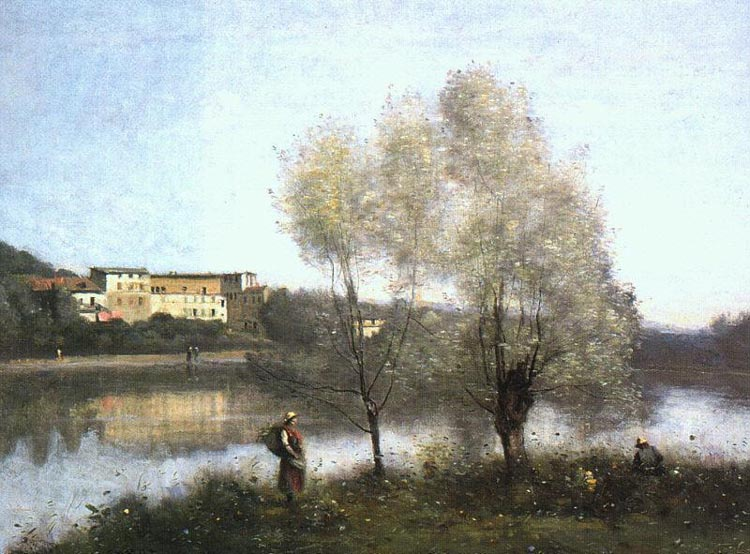
\includegraphics[width=.8\textwidth]{corotavray}
\caption[Jean-Baptiste Corot. \textit{Ville d'Avray} (ca. 1867).]{Jean-Baptiste Corot. \textit{Ville d'Avray} (ca. 1867).
Fonte: Wikipedia (\url{http://fr.wikipedia.org/wiki/Fichier:Corot.villedavray.750pix.jpg})}
\label{corot}
\end{figure}

O comando \verb+\caption{...}+ gera o rótulo da figura (ou tabela).

\section{Rótulos ao lado da figura (side captions)}

Use o pacote sidecap:

\begin{verbatim}
\usepackage{sidecap}
\end{verbatim}

E o ambiente SCfigure ao invés de figure (figura \ref{moreau}).

\begin{verbatim}
\begin{SCfigure}
\centering
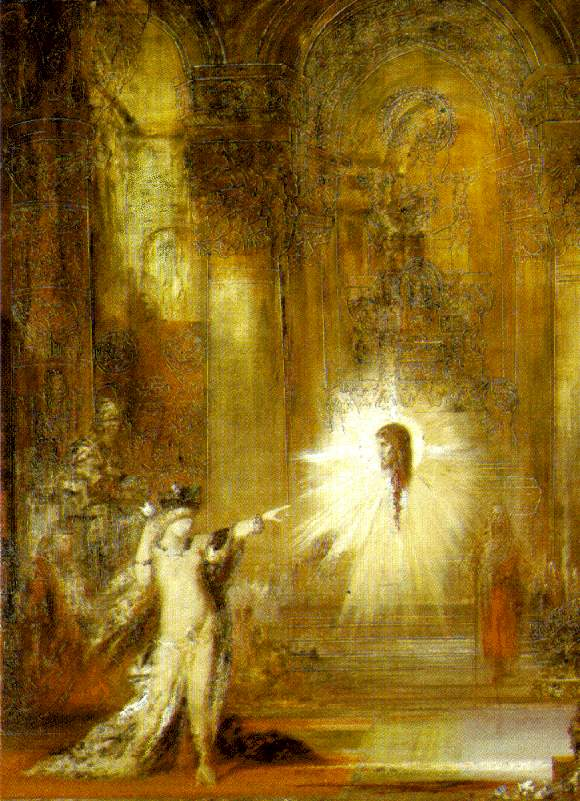
\includegraphics[width=.4\textwidth]{moreau-apparition}
\caption{\textit{L'apparition}, de Gustave Moreau (1875).}
\label{moreau}
\end{SCfigure}
\end{verbatim}


\begin{SCfigure}
\centering
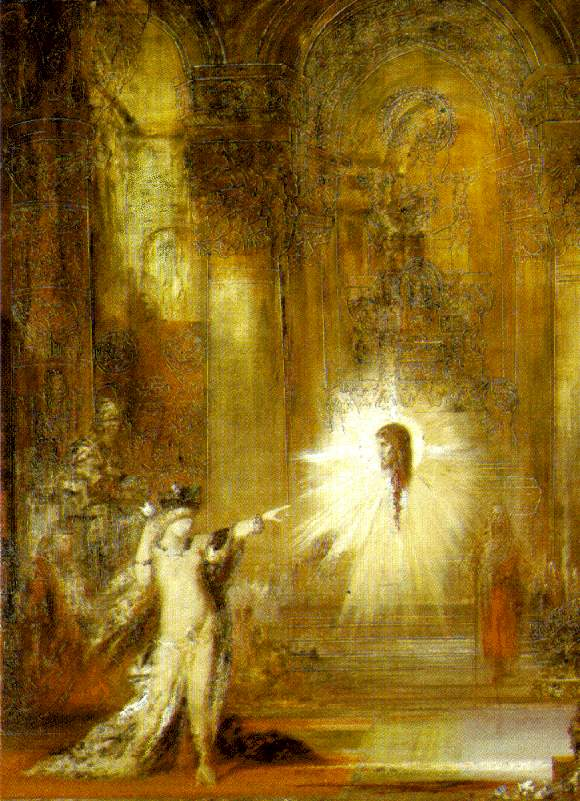
\includegraphics[width=.4\textwidth]{moreau-apparition}
\caption{\textit{L'apparition}, de Gustave Moreau (1875).}
\label{moreau}
\end{SCfigure}


\section{Figuras dentro de figuras (subfloats)}

Usando o pacote \texttt{subfig}, você pode incluir figuras dentro de outras figuras. 

As figuras serão colocadas lado a lado; se não houver espaço, vão para a linha inferior. Para colocar uma subfigura manualmente embaixo, é só inserir a marcação de novo parágrafo (\textbackslash\textbackslash).

Para inserir espaços entre as figuras, use um dos comandos:

\begin{itemize}
\item Espaços brancos, backspaces ou tabs produzirão um espaço regular;
\item Espaços matemáticos: \verb+\qquad, \quad, \;,  \,+
\item Espaço genérico: \verb+\hspace{Xcm}+;
\item Espaço expandido/contraído automaticamente: \verb+\hfill+
\end{itemize}

Exemplo:\footnote{\url{http://en.wikibooks.org/wiki/LaTeX/Floats,\_Figures\_and\_Captions#Subfloats}}

\begin{verbatim}
\usepackage{subfig}
 
\begin{figure}
  \centering
  \subfloat[A gull]{\label{fig:gull}\includegraphics[width=0.3\textwidth]{gull}}                
  \subfloat[A tiger]{\label{fig:tiger}\includegraphics[width=0.3\textwidth]{tiger}}
  \subfloat[A mouse]{\label{fig:mouse}\includegraphics[width=0.3\textwidth]{mouse}}
  \caption{Pictures of animals}
  \label{fig:animals}
\end{figure}
\end{verbatim}


\begin{center}
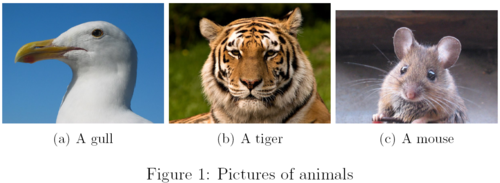
\includegraphics[width=0.5\textwidth]{subfig.png}
\end{center}

\section{Figuras lado-a-lado}
\begin{english}

Source:
\url{http://theoval.cmp.uea.ac.uk/~nlct/latex/novices/sidebyside.html}

The figure environment, should really be called "figures" rather than "figure", as you can have more than one \verb+\caption+ command within the environment, however, since the contents of the figure environment can't have a page break, nor can the figures within a single figure environment float independently of each other, it is more usual to have a separate figure environment for each figure. As a result, people tend to forget that they can have more than one figure in a figure environment, which gives rise to the frequently asked question "how can I have side-by-side figures?"

The answer to this is to put the two figures in the same figure environment. To do this, we can use the minipage environment, which was covered earlier. Recall that the minipage environment creates a horizontal box, which means that two mini-pages can be placed side-by-side on the same line. All you need to do now, is place one image and caption in one mini-page, and the other image and caption in the neighbouring mini-page:

\begin{verbatim}
\begin{figure}[htbp]
\begin{minipage}{0.5\linewidth}
\centering
\includegraphics{circle}
\caption{A Circle}
\label{fig:circle}
\end{minipage}%
\begin{minipage}{0.5\linewidth}
\centering
\includegraphics{rectangle}
\caption{A Rectangle}
\label{fig:rectangle}
\end{minipage}
\end{figure}
\end{verbatim}

\end{english}

\section{Figuras com o tamanho da página em textos de duas colunas}

É só colocar um * na frente de \texttt{figure}: 

\begin{verbatim}
\begin{figure*}
\end{figure*}
\end{verbatim}

Assim, ela vai ter a largura das duas colunas.



\chapter{Referências}

\section{Referências cruzadas}
O \LaTeX{} pode inserir referências cruzadas em praticamente qualquer parte do texto. Primeiro, insere-se um rótulo (label):

\begin{verbatim}
\label{latexbasico}
\end{verbatim}

Depois, podemos nos referir ao marcador/rótulo com os comandos:

\begin{verbatim}
\ref{latexbasico}
\end{verbatim}

\begin{verbatim}
\pageref{latexbasico}
\end{verbatim}

O primeiro refere-se à seção, o outro, à página. Assim, inserindo um \verb+\label{...}+ numa parte do texto, em qualquer outra parte podemos nos referir a ela. Veja este exemplo: é a figura \ref{latexbasico} na página \pageref{latexbasico}. Eu nem tenho ideia em que página ou seção está, o programa simplesmente vai mostrar no texto final, como neste caso: 

\begin{quote}
A concepção da figura feminina na pintura do simbolista  Gustave Moreau (figura \ref{moreau}), pode ser contrastada com a interpretação realista de Courbet (figura \ref{courbet}, p. \pageref{courbet}).
\end{quote}

Podemos facilmente fazer referências a tabelas, seções, capítulos, figuras etc. E eu posso mudar essa citação de página à vontade, sempre que eu compilar o texto, a paginação e a referência vão aparecer corretas. O único porém é que nem sempre as referências aparecem na primeira vez em que se roda o programa. Simplesmente compile o documento novamente, e se necessário, outra vez.

\section{Hyperlinks}
Se quiser hyperlinks clicáveis no seu pdf, use o comando \verb+\url{}+:



\begin{minipage}{.5\textwidth}
\begin{verbatim}
\url{www.wikipedia.org}
\end{verbatim}
\end{minipage}
\url{www.wikipedia.org}





\chapter{Cores}
Para texto ou outros elementos coloridos, use um dos pacotes: \texttt{color} ou \texttt{xcolor}.

A sintaxe é simples:
\begin{verbatim}
\textcolor{nome da cor}{Texto nessa cor}
\end{verbatim}

\begin{table}[h!]
\caption{As 68 cores da opção \texttt{dvipsnames}}
\label{cores}
\centering
\sffamily
\begin{tabular}{llll} 

 {\color{Apricot} Apricot}& 
 {\color{Aquamarine} Aquamarine}& 
 {\color{Bittersweet} Bittersweet}& 
 {\color{Black} Black}\\  
 {\color{Blue} Blue}& 
 {\color{BlueGreen} BlueGreen}& 
 {\color{BlueViolet} BlueViolet}& 
 {\color{BrickRed} BrickRed}\\ 
 {\color{Brown} Brown}& 
 {\color{BurntOrange} BurntOrange}& 
 {\color{CadetBlue} CadetBlue}& 
 {\color{CarnationPink} CarnationPink}\\ 
 {\color{Cerulean} Cerulean}& 
 {\color{CornflowerBlue} CornflowerBlue}& 
 {\color{Cyan} Cyan}& 
 {\color{Dandelion} Dandelion}\\ 
 {\color{DarkOrchid} DarkOrchid}& 
 {\color{Emerald} Emerald}& 
 {\color{ForestGreen} ForestGreen}& 
 {\color{Fuchsia} Fuchsia}\\ 
 {\color{Goldenrod} Goldenrod}& 
 {\color{Gray} Gray}& 
 {\color{Green} Green}& 
 {\color{GreenYellow} GreenYellow}\\ 
 {\color{JungleGreen} JungleGreen}& 
 {\color{Lavender} Lavender}& 
 {\color{LimeGreen} LimeGreen}& 
 {\color{Magenta} Magenta}\\ 
 {\color{Mahogany} Mahogany}& 
 {\color{Maroon} Maroon}& 
 {\color{Melon} Melon}& 
 {\color{MidnightBlue} MidnightBlue}\\ 
 {\color{Mulberry} Mulberry}& 
 {\color{NavyBlue} NavyBlue}& 
 {\color{OliveGreen} OliveGreen}& 
 {\color{Orange} Orange}\\ 
 {\color{OrangeRed} OrangeRed}& 
 {\color{Orchid} Orchid}& 
 {\color{Peach} Peach}& 
 {\color{Periwinkle} Periwinkle}\\ 
 {\color{PineGreen} PineGreen}& 
 {\color{Plum} Plum}& 
 {\color{ProcessBlue} ProcessBlue}& 
 {\color{Purple} Purple}\\  
 {\color{RawSienna} RawSienna}& 
 {\color{Red} Red}& 
 {\color{RedOrange} RedOrange}& 
 {\color{RedViolet} RedViolet}\\ 
 {\color{Rhodamine} Rhodamine}& 
 {\color{RoyalBlue} RoyalBlue}& 
 {\color{RoyalPurple} RoyalPurple}& 
 {\color{RubineRed} RubineRed}\\
 {\color{Salmon} Salmon}& 
 {\color{SeaGreen} SeaGreen}& 
 {\color{Sepia} Sepia}& 
 {\color{SkyBlue} SkyBlue}\\ 
 {\color{SpringGreen} SpringGreen}& 
 {\color{Tan} Tan}& 
 {\color{TealBlue} TealBlue}& 
 {\color{Thistle} Thistle}\\
 {\color{Turquoise} Turquoise}& 
 {\color{Violet} Violet}& 
 {\color{VioletRed} VioletRed}& 
 {\color{White} White} (White)\\
 {\color{WildStrawberry} WildStrawberry}& 
 {\color{Yellow} Yellow}& 
 {\color{YellowGreen} YellowGreen}& 
 {\color{YellowOrange} YellowOrange}\\
 \end{tabular} 
\end{table}


Usando a opção dvipsnames (\verb+\usepackage[dvipsnames]{xcolor}+), temos 68 opções de cores (ver tabela \ref{cores}). Para outras opções, ver a documentação do pacote \texttt{xcolor}.






\chapter{Fontes}
\label{fontes}
Para selecionar uma fonte que não é a padrão (Computer Modern), você precisa incluir um pacote de fontes nativo ou usar o pacote \texttt{fontspec} e compilar com o comando \texttt{xelatex}.

\begin{verbatim}
 \usepackage[T1]{fontenc}
 \usepackage{times}
\end{verbatim}
 
 No caso, \texttt{times} é o pacote da fonte (Times, igual à Times New Roman). Há dezenas desses pacotes, muitos vêm direto na instalação básica do \LaTeX. Você pode encontrá-las em: \url{http://www.tug.dk/FontCatalogue/}. Há muitas fontes interessantes, boas e legíveis, e todas elas podem ser utilizadas compilando o documento com o comando: \textsf{pdflatex (nome do documento).tex} (ou direto no editor de texto). Por exemplo, temos as fontes: Charter, Palatino, Utopia, Century... Mas se você quiser usar as fontes que vêm com seu computador, você tem que compilar o texto com \texttt{xelatex (nome do documento).tex}.
 
 \section{O pacote \texttt{fontspec}}
 O pacote \texttt{fontspec} facilita a escolha de fontes não nativas ao Latex. O arquivo deve ser compilado com o comando \texttt{xelatex (nomedoarquivo.tex)}, 
 
 
 \begin{verbatim}
\usepackage{fontspec}
\defaultfontfeatures{Ligatures={TeX}}
\setromanfont{Chaparral Pro}
\setsansfont{Chaparral Pro}
\setmonofont[Scale=MatchLowercase]{Consolas}
 \end{verbatim}
 

O comando

\begin{verbatim}
\defaultfontfeatures{Ligatures={TeX}}
\end{verbatim}


faz com que conjuntos de caracteres LaTeX como \verb+---+ e \verb+``+ apareçam como ---~ e ``~ no texto final. 

Depois temos a definição da fonte serifada, sem serifa (geralmente usada para títulos) e  monoespaçada: 

\begin{verbatim}
\setromanfont{Chaparral Pro}
\setsansfont{Chaparral Pro}
\setmonofont[Scale=MatchLowercase]{Consolas}
\end{verbatim} 

Claro que você pode (ou deve) substituir o nome das fontes pelas que mais preferir. Com o Adobe Acrobat Reader, vêm as fontes de graça: Minion Pro e Myriad Pro.\footnote{Para Linux, faça o download de: \url{http://www.adobe.com/support/downloads/detail.jsp?ftpID=4426}, extraia e instale. Para Windows, vá até a pasta onde instalou o Reader (Arquivos de Programas), procure as fontes e instale.} Outra fonte interessante é \href{http://scripts.sil.org/cms/scripts/page.php?site\_id=nrsi\&id=Gentium\_download}{Gentium}. 

\chapter{Idiomas}
\label{idiomas}

Para definir a língua em Latex, usa-se o pacote \texttt{babel} para compilar em \texttt{pdflatex} e o pacote \texttt{polyglossia} para compilar em xelatex. São esses dois pacotes, em cada caso, que definem as línguas.\footnote{Pode-se usar também o pacote \texttt{babel} com \texttt{xelatex}, mas somente para línguas ocidentais.} A mudança de uma língua para a outra afeta coisas que são automáticas no Latex: abstract, títulos de capítulos, sumário, datas, hifenização, etc. Há uma diferença de preâmbulo, de acordo com o caso. 

Para \texttt{pdflatex}:

\begin{verbatim}
\documentclass[12pt,a4paper]{article}
\usepackage[brazil]{babel} %escolha da língua com pacote babel
\usepackage[utf8]{inputenc} %para inserir acentos
\usepackage[T1]{fontenc}
\usepackage{lmodern} %pacote de fonte
\end{verbatim}

Pode-se também escolher mais de uma língua, e no caso a última língua será a língua ativa:

\begin{verbatim}
\usepackage[english,brazil]{package}
\end{verbatim}

Nesse caso, escolhe-se a língua ativa com o ambiente

\begin{verbatim}
\begin{otherlanguage}{english}
...
\end{otherlanguage}
\end{verbatim}

sendo que a língua-padrão do documento será a última (português do Brasil).

Com o pacote \texttt{polyglossia}:

\begin{verbatim}
 \usepackage{polyglossia}
 \setmainlanguage{brazil}
 \setotherlanguages{french,english,german,arabic}
 \newfontfamily\arabicfont[Script=Arabic]{Adobe Arabic}
\end{verbatim} 

Podemos fazer isso facilmente com um ambiente:

\begin{verbatim}
\begin{french}
...
\end{french}
\end{verbatim}

ou então simplesmente: \verb+\textfrench{...}+.


A vantagem do pacote \texttt{polyglossia} é que é possível inserir mais facilmente textos em várias línguas:
\medskip


\begin{tabular}{ll}
\begin{minipage}{.5\textwidth}
\begin{verbatim}
\begin{english}
Texto em inglês.
\end{english}
\end{verbatim}
\end{minipage}
&
\begin{minipage}{.5\textwidth}
\begin{verbatim}
\textenglish{Texto em inglês}
\end{verbatim}
\end{minipage}
\end{tabular}

\medskip



\section{Alfabetos não latinos e escritas não ocidentais}

Para textos em outros alfabetos ou sistemas de escrita, sem se preocupar com hifenização ou composição de documentos completos, é mais fácil definir a fonte, se a própria fonte que estiver usando não tiver os caracteres. Assim, se estiver escrevendo texto que contenha caracteres gregos, cirílicos etc., use em todo o documento uma fonte que já tenha todos esses caracteres.Então eu posso simplesmente escrever:

\medskip


%\begin{tabularx}{1.0\textwidth}{XX}

\begin{mdframed}[backgroundcolor=lightgray]

\textit{Texto em russo:}
\medskip

\begin{russian}
Лев Николаевич Толстой (28 августа (9 сентября) 1828, Ясная Поляна, Тульская губерния, Российская империя — 7 (20) ноября 1910, станция Астапово, Тамбовская губерния, Российская империя), граф — один из наиболее широко известных русских писателей и мыслителей. (\url{http://ru.wikipedia.org/wiki/Толстой,\_Лев\_Николаевич})
\end{russian} 
\end{mdframed}


\medskip

\begin{mdframed}[backgroundcolor=lightgray]
\textit{Texto em grego:}
\medskip

\begin{greek}
Ο Οδυσσέας Ελύτης (2 Νοεμβρίου 1911 - 18 Μαρτίου 1996), φιλολογικό ψευδώνυμο του Οδυσσέα Αλεπουδέλλη του Παναγιώτη, ήταν ένας από τους σημαντικότερους Έλληνες ποιητές, μέλος της λογοτεχνικής γενιάς του '30.
\end{greek}
%\end{tabularx}
\end{mdframed}



\medskip

Se a fonte que eu estiver usando não tiver os caracteres de uma determinada língua, posso definir outra fonte para essa língua usando os comandos:

%No caso deste documento, estou usando a fonte Stempel Garamond, então defino outra fonte para ser usada por outras línguas:

\begin{verbatim}
\newfontfamily\russianfont[Script=Cyrillic]{Minion Pro}
\newfontfamily\greekfont[Script=Greek]{Minion Pro} 
\end{verbatim}

%Mas se eu já estiver usando a fonte Minion (ou outra que tenha esses caracteres), não preciso de me preocupar em mudar.\footnote{Programas de processamento de texto como o Word fazem isso automaticamente: se a fonte que está usando não tem caracteres em japonês, por exemplo, ele mudará automaticamente para uma que tem.} 

Para escritas não ocidentais também utilizamos o pacote \texttt{fontspe}c e/ou o pacote \texttt{polyglossia}


\begin{center}
\begin{verbatim}
\usepackage{polyglossia}
\setotherlanguage{arabic}
\usepackage{fontspec}
\usepackage{arabxetex}
\newfontfamily\arabicfont[Script=Arabic]{Adobe Arabic}
\begin{arab}
 (texto em árabe)
\end{arab}
\end{verbatim}
\end{center}


\begin{center}
\begin{arab}
 العربية أكثر لغات المجموعة السامية متحدثين

\end{arab}

\end{center}

\medspace

O pacote \texttt{arabxetex} usa automaticamente a fonte gratuita Scheherazade, mas, como no exemplo, pode ser especificada qualquer fonte com suporte a árabe/persa/urdu.

Para escrever em chinês, japonês ou coreano, utilizamos o pacote \texttt{xeCJK}:\footnote{A solução para um texto com os três sistemas (chinês, japonês e coreano) foi copiada de: \url{http://tex.stackexchange.com/questions/45331/combining-chinese-japanese-and-korean-text-with-xecjk}}
\label{japones}
\medskip


\begin{verbatim}
\usepackage{xeCJK}
\setCJKfamilyfont{zhrm}{SimSun}
\setCJKfamilyfont{jarm}{MS Mincho}
\setCJKfamilyfont{korm}{Batang}

\newcommand\Chinese{\renewcommand\CJKrmdefault{zhrm}\CJKnospace\normalfont}
\newcommand\Japanese{\renewcommand\CJKrmdefault{jarm}\CJKnospace\normalfont}
\newcommand\Korean{\renewcommand\CJKrmdefault{korm}\CJKspace\normalfont}
...
\begin{tabular}{ccc}
{\Japanese おはよう}
 & Ohayo! & ``Bom dia!" em japonês\\

{\Chinese 早安} & Zǎo ān! & "Bom dia!" em chinês\\

{\Korean 안녕하세요}   &  An-nyeong-ha-se-yo & "Como vai?"/"Bom dia!" em coreano.
\end{tabular}
\end{verbatim}

\medskip


\begin{center}
\begin{tabular}{ccc}
{\Japanese おはよう}
 & Ohayo! & ``Bom dia!" em japonês\\

{\Chinese 早安} & Zao an! & ``Bom dia!" em chinês\\

{\Korean 안녕하세요}   &  An-nyeong-ha-se-yo & ``Como vai?"/"Bom dia!" em coreano.

\end{tabular}

\end{center}

Se você for escrever textos em somente uma dessas línguas, é bem mais simples escolher só uma delas:

\begin{verbatim}
\setCJKmainfont{Batang} %para coreano
\end{verbatim}



Mais informações podem ser obtidas com a documentação dos pacotes \texttt{fontspec} e \texttt{po\-ly\-glos\-sia}. 


\chapter{Documentos técnicos e científicos brasileiros com abnTeX2}

O abn\TeX 2, evolução do abn\TeX{} (''Absurd Norms for TeX"), é uma suíte composta por uma classe e por pacotes de citação e de formatação de estilos bibliográficos para \LaTeX{} que atendem os requisitos das normas da ABNT (Associação Brasileira de Normas Técnicas) para elaboração de documentos técnicos e científicos brasileiros, como artigos científicos, relatórios técnicos, trabalhos acadêmicos como teses, dissertações, projetos de pesquisa e outros documentos do gênero. (Este documento não foi escrito sob o modelo do abn\TeX, nem segue os
padrões da ABNT.)

A primeira versão do abnTeX2 foi concluída em dezembro de 2012 e disponibilizada ao público no dia 20 daquele mês. O abnTeX2 foi disponibilizado ao CTAN, "The Comprehensive TEX Archive Network", em 2 de janeiro de 2013 e pode ser consultado em \url{http://www.ctan.org/pkg/abntex2}. O abnTeX2 foi a primeira contribuição brasileira ao repositório mundial de classes e pacotes de LaTeX do CTAN, e está disponível nas principais distribuições \LaTeX --- \TeX Live, Mik\TeX, Mac\TeX{} e pro\TeX t. 

O software é mantido desde então por Lauro César Araujo e pela comunidade de indivíduos e de organizações que adotam e/ou investem em software livre, como o Centro de Pesquisa em Arquitetura da Informação (CPAI/UnB). O projeto é hospedado em: \url{http://code.google.com/p/abntex2/}. 

A instalação da classe abn\TeX 2 é simples, semelhante a outros pacotes ou classes (ver seção \ref{pacotes}). Instruções detalhadas para vários sistemas e distribuições podem ser encontradas em: \url{https://code.google.com/p/abntex2/wiki/Instalacao}.

A suíte abn\TeX 2 é composta por três elementos principais:\footnote{Somam-se a
esses elementos a documentação e os modelos (disponíveis em: \url{https://code.google.com/p/abntex2/downloads/list}), todos distribuídos de forma
conjunta.}

\begin{itemize}
  \item a classe de formação de trabalhos acadêmicos \textsf{abntex2}, descrita
  neste manual;
  \item o pacote de citações bibliográficas \texttt{abntex2cite}; e
  \item as especificações de formatação de referências bibliográficas
  \texttt{abntex2-num.bst} e \texttt{abntex2-alf.sty}.
\end{itemize}

O abnTeX2 foi desenvolvido com base nos requisitos das seguintes normas ABNT:

\begin{description}
  \item[ABNT NBR 6022:2003] Informação e documentação - Artigo em publicação
  periódica científica impressa - Apresentação
  \item[ABNT NBR 6023:2000] Informação e documentação - Referência -
  Elaboração\footnote{A versão corrente da ABNT NBR 6023 é a 6023:2002. Porém,
  até este momento, o abnTeX2 traz os estilos compatíveis com a versão
  anterior da norma. A atualização dos estilos é uma das etapas posteriores do
  projeto. Consulte a documentação do pacote \texttt{abntex2cite} \texttt{abntex2cite-alf}
  para mais informações.}
  \item[ABNT NBR 6024:2012] Informação e documentação - Numeração
  progressiva das seções de um documento - Apresentação
  \item[ABNT NBR 6027:2003] Informação e documentação - Sumário -
  Apresentação
  \item[ABNT NBR 6028:2003] Informação e documentação - Resumo -
  Apresentação
  \item[ABNT NBR 6034:2004] Informação e documentação - Índice -
  Apresentação
  \item[ABNT NBR 10520:2002] Informação e documentação - Citações
  \item[ABNT NBR 10719-2011] Informação e documentação - Relatório técnico
  e-ou científico - Apresentação
  \item[ABNT NBR 14724:2011] Informação e documentação - Trabalhos
  acadêmicos - Apresentação
  \item[ABNT NBR 15287:2011] Informação e documentação - Projeto de pesquisa -
  Apresentação
\end{description}

A classe \textsf{abntex2} foi criada como um conjunto de configurações da classe
\textsf{memoir}\footnote{A versão anterior do abntex era baseada na
classe \textsf{report}.}. Desse modo, todas as opções do \textsf{memoir} estão
disponíveis, como por exemplo, |12pt,openright,twoside,a4paper,artile|. Consulte
o manual do \textsf{memoir} para outras opções.

As opções mais comuns de inicialização do texto de um trabalho segundo as normas da ABNT são:

\begin{verbatim}
   \documentclass[12pt,openright,twoside,a4paper]{abntex2}
\end{verbatim}

É interessante observar que a ABNT NBR 14724:2011 (seção 5.1) recomenda que os
trabalhos sejam impressos no anverso e no verso das folhas. Isso é obtido com a
opção \texttt{twoside}. 

A opção \verb+article+ é útil para produção de artigos com abn\TeX 2.
Nesse caso, a maioria dos elementos pré-textuais se tornam desnecessários. A macro \verb+\part+ também é permitida com a opção\texttt{article}. Quando esta opção for
utilizada, a classe \texttt{abntex2} não forçará quebra de página para os
elementos pré-textuais e definirá a formatação do capítulo de forma idêntica à
formatação das seções. Por padrão, quando a opção \texttt{article} estiver presente,
você deve iniciar as divisões do trabalho com \verb+\section+, e não \verb+\chapter+, como
é usual em trabalhos monográficos. Porém, caso queira iniciar as divisões com
\verb+\chapter+ ao invés de \verb+\section+, adicione as linhas abaixo no preâmbulo do
documento para que a numeração dos capítulos, seções, figuras e tabelas sejam
corretamente sequenciados:

\begin{verbatim}
  \counterwithout{section}{section}
  \counterwithout{figure}{chapter}
  \counterwithout{table}{chapter}
\end{verbatim}

O abn\TeX{} está programado para utilizar seja o compilador \texttt{pdflatex}, fazendo uso dos pacotes \texttt{babel} e \texttt{inputenc} (utf8) e fontes nativas do \LaTeX, ou então o compilador \texttt{xelatex}, fazendo uso do pacote \texttt{polyglossia} e \texttt{fontspec}, para uso de fontes TrueType e OpenType (ver capítulos \ref{fontes} e \ref{idiomas}).

\section{Macros de dados do trabalho}\label{sec-macrosdados}
O uso das macros do abntex é bastante intuitivo, seguindo a filosofia do Latex de não deixar o autor se preocupar com a formatação. As macros são bastante autoexplicativas:

\begin{verbatim}
\titulo{}

\autor{}

\local{}

\data{}

\orientador{}

\coorientador{}

\instituicao{}

\tipotrabalho{}

\preambulo{}

\imprimircapa

\imprimirfolhaderosto

...

\apendices

\anexos 

\end{verbatim}



Abaixo um exemplo do Modelo de Trabalho Acadêmico do abnTeX:


\begin{verbatim}
% ---
% Informações de dados para CAPA e FOLHA DE ROSTO
% ---
\titulo{Modelo Canônico de\\ Trabalho Acadêmico com \abnTeX}
\autor{Equipe \abnTeX}
\local{Brasil}
\data{2013, v-1.3}
\orientador{Lauro César Araujo}
\coorientador{Equipe \abnTeX}
\instituicao{%
  Universidade do Brasil -- UBr
  \par
  Faculdade de Arquitetura da Informação
  \par
  Programa de Pós-Graduação}
\tipotrabalho{Tese (Doutorado)}
% O preambulo deve conter o tipo do trabalho, o objetivo, 
% o nome da instituição e a área de concentração 
\preambulo{Modelo canônico de trabalho monográfico acadêmico em conformidade com
as normas ABNT apresentado à comunidade de usuários \LaTeX.}


% ----------------------------------------------------------
% ELEMENTOS PRÉ-TEXTUAIS
% ----------------------------------------------------------
% \pretextual

% ---
% Capa
% ---
\imprimircapa
% ---

% ---
% Folha de rosto
% (o * indica que haverá a ficha bibliográfica)
% ---
\imprimirfolhaderosto*

\end{verbatim}

Ambientes abnTeX (a ser colocados entre \verb+\begin{*nome do ambiente*}+
\verb+\end{*nome do ambiente*}+):


\begin{multicols}{3}
\begin{itemize}
\item errata \item folhadeaprovacao \item dedicatoria \item agradecimentos \item epigrafe
\item resumo \item resumo[Abstract] \item listoffigures \item listoftables \item tableofcontents
\end{itemize}
\end{multicols}

Para mais informações e detalhes, referir-se à documentação do projeto abn\TeX 2: \url{http://code.google.com/p/abntex2/downloads/list}.


\chapter{Outros recursos}

\begin{itemize}
\item Para informações sobre tipografia, ver o livro: 
\href{http://www.amazon.com/Elements-Typographic-Style-Robert-Bringhurst/dp/0881791326}{\textit{The Elements of Typographic Style}}, de Robert Bringhurst. 
\item
Para exemplos de como funciona a tipografia no \LaTeX, ver: \url{http://nitens.org/taraborelli/latex}. 
\item
Para modelos de currículos, ver: \url{http://nitens.org/taraborelli/cvtex}.
\item Para sanar suas dúvidas, há um excelente fórum de usuários Latex em: \url{http://tex.stackexchange.com}
\end{itemize}



\addpart{Apêndices}

\chapter*{Números de página na borda}
\begin{verbatim}
\setlength{\footskip}{0pt}
\rofoot[\centerpageno{o}]{\centerpageno{o}}
\lefoot[\centerpageno{e}]{\centerpageno{e}}
\def\centerpageno#1{\leavevmode
  \vbox to 0pt{
    \vss
    \hbox to 0pt{\large\normalfont
      \if#1o\kern 2em\else\hss\fi\thepage
      \if#1o\hss\else\kern2em\fi}
    \vskip.5\textheight
    \vskip\baselineskip}}
\end{verbatim}

Esses comandos acima são para colocar o número da página na borda.

Também pode colocar:  \verb+\fbox{\thepage}+ para número de página dentro de quadrado.

Obs: só funciona com classe koma-script e e pacote scrpage2.


\chapter*{Caixas de texto}

Se você quiser colocar parte do texto dentro de um quadro, a maneira mais fácil é usar o pacote \texttt{framed} (\verb+\usepackage{framed}+) e o pacote \texttt{xcolor}. O texto dentro do quadro pode ser maior que uma linha, parágrafo ou página, inclusive com cor de fundo. Usando os ambientes \texttt{framed} ou \texttt{shaded} ou \texttt{snugshade}, você pode escrever vários parágrafos dentro da caixa. 



Uso:

\medskip
\medskip

\footnotesize{
\begin{tabular}{p{6cm}p{5cm}p{5cm}}
\verb+\definecolor{shadecolor}{Gray}{10.0}+ & Define a cor da sombra (fundo) &  \\
\verb+\begin{framed} Uma história... \end{framed}+ & Bordas ao redor do texto & \begin{framed} Uma história... \end{framed}\\
\verb+\begin{shaded} Uma história... \end{shaded}+ & Texto com sombra de fundo & \begin{shaded} Uma história... \end{shaded}\\
\verb+\begin{snugshade} Uma história... \end{snugshade}+ & Texto com sombra de fundo mais justa. & \colorbox{Gray}{Uma história\ldots}\\
\verb+\fcolorbox{Magenta}{Gray}{Uma história...}+ & Define a cor da borda e a cor do fundo. Necessário pacote \texttt{xcolor}.& \fcolorbox{Magenta}{Gray}{Uma história...} \\
\verb+\colorbox{Gray}{Uma história…}+ & Um sombreado só do tamanho do texto. & \colorbox{Gray}{Uma história\ldots}\\
\verb+\framebox{Uma história\ldots}+ & Uma caixa ao redor do texto do tamanho do parágrafo. & \framebox{Uma história\ldots}\\
\verb+\fbox{Uma história\ldots}+ & Uma caixa ao redor do texto do tamanho do texto. & \fbox{Uma história\ldots}\\
\end{tabular}
}

\medskip

O pacote \texttt{mdframed} é bom para fazer caixas coloridas com texto de mais de uma linha ou parágrafo. Você pode especificar diretamente a cor de fundo, e outras características.

Exemplo:

\vspace{-1em}
\begin{verbatim}
\begin{mdframed}[backgroundcolor=lightgray]
...
\end{mdframed}
\end{verbatim}

\begin{mdframed}[backgroundcolor=lightgray]
I. Quo usque tandem abutere, Catilina, patientia nostra? quam diu etiam furor iste tuus nos eludet? quem ad finem sese effrenata iactabit audacia? Nihilne te nocturnum praesidium Palati, nihil urbis vigiliae, nihil timor populi, nihil concursus bonorum omnium, nihil hic munitissimus habendi senatus locus, nihil horum ora voltusque moverunt? Patere tua consilia non sentis, constrictam iam horum omnium scientia teneri coniurationem tuam non vides? Quid proxima, quid superiore nocte egeris, ubi fueris, quos convocaveris, quid consilii ceperis, quem nostrum ignorare arbitraris? \hfill ---Cicero, \textit{Oratio in L. Catilinam Prima}.

\end{mdframed}

\chapter*{Uma entrada de capítulo elaborada}
Estilo de capítulo “Veelo”, da classe \texttt{memoir}.

\begin{verbatim}
\usepackage{titlesec}
\titleformat{\chapter}[display]
{\normalfont\Large\raggedleft}
{\MakeUppercase{\chaptertitlename}%
\rlap{ \resizebox{!}{1.5cm}{\thechapter} \rule{5cm}{1.5cm}}}
{10pt}{\Huge}
\titlespacing*{\chapter}{0pt}{30pt}{20pt}
\end{verbatim}


\chapter*{Usando Xe\LaTeX{} e as classes Tufte-\LaTeX{}}

Se você quiser usar um estilo parecido com o dos livros de E. Tufte, as classes \texttt{tufte-handout} (para artigos) e \texttt{tufte-book} (para livros) são uma opção interessante para sair da mesmice. Mas se quiser compilar com \texttt{xelatex} para usar as fontes do sistema, deve usar o código abaixo no preâmbulo para fazer os cabeçalhos das páginas funcionarem direito:

\begin{verbatim}
\renewcommand{\allcapsspacing}[1]{{\addfontfeature{LetterSpace=20.0}#1}}
\renewcommand{\smallcapsspacing}[1]{{\addfontfeature{LetterSpace=5.0}#1}}
\renewcommand{\textsc}[1]{\smallcapsspacing{\textsmallcaps{#1}}}
\renewcommand{\smallcaps}[1]{\smallcapsspacing{\scshape\MakeTextLowercase{#1}}}
\end{verbatim}


%\chapter{Um sumário diferente}
%O código abaixo gera um sumário mais elaborado, com cores e números de página diferenciados. 
%
%\begin{verbatim}
%\documentclass{book}
%\usepackage{xcolor}
%\usepackage{framed}
%\usepackage{tikz}
%\usepackage{titletoc}
%\usepackage{etoolbox}
%\usepackage{polyglossia}
%\setmainlanguage{brazil}
%\usepackage{fontspec}
%\defaultfontfeatures{Ligatures={TeX}}
%\setmainfont{New Caledonia LT Std}
%\setsansfont{New Caledonia LT Std}
%\setmonofont[Scale=MatchLowercase]{Menlo}
%%\usepackage[bookmarks]{hyperref}
%
%% definition of some personal colors
%\definecolor{myred}{RGB}{127,0,0}
%\definecolor{myyellow}{RGB}{169,121,69}
%
%% command for the circle for the number of part entries
%\newcommand\Circle[1]{\tikz[overlay,remember picture] 
%  \node[draw,circle, text width=18pt,line width=1pt] {#1};}
%
%% patching of \tableofcontents to use sans serif font for the tile
%\patchcmd{\tableofcontents}{\contentsname}{\sffamily\contentsname}{}{}
%% patching of \@part to typeset the part number inside a framed box in its own line
%% and to add color
%\makeatletter
%\patchcmd{\@part}
%  {\addcontentsline{toc}{part}{\thepart\hspace{1em}#1}}
%  {\addtocontents{toc}{\protect\addvspace{20pt}}
%    \addcontentsline{toc}{part}{\huge{\protect\color{myyellow}%
%      \setlength\fboxrule{2pt}\protect\Circle{%
%        \hfil\thepart\hfil%
%      }%
%    }\\[2ex]\color{myred}\sffamily#1}}{}{}
%
%%\patchcmd{\@part}
%%  {\addcontentsline{toc}{part}{\thepart\hspace{1em}#1}}
%%  {\addtocontents{toc}{\protect\addvspace{20pt}}
%%    \addcontentsline{toc}{part}{\huge{\protect\color{myyellow}%
%%      \setlength\fboxrule{2pt}\protect\fbox{\protect\parbox[c][1em][c]{1.5em}{%
%%        \hfil\thepart\hfil%
%%      }}%
%%    }\\[2ex]\color{myred}\sffamily#1}}{}{}
%\makeatother
%
%% this is the environment used to typeset the chapter entries in the ToC
%% it is a modification of the leftbar environment of the framed package
%\renewenvironment{leftbar}
%  {\def\FrameCommand{\hspace{6em}%
%    {\color{myyellow}\vrule width 2pt depth 6pt}\hspace{1em}}%
%    \MakeFramed{\parshape 1 0cm \dimexpr\textwidth-6em\relax\FrameRestore}\vskip2pt%
%  }
% {\endMakeFramed}
%
%% using titletoc we redefine the ToC entries for parts, chapters, sections, and subsections
%\titlecontents{part}
%  [0em]{\centering}
%  {\contentslabel}
%  {}{}
%\titlecontents{chapter}
%  [0em]{\vspace*{2\baselineskip}}
%  {\parbox{4.5em}{%
%    \hfill\Huge\sffamily\bfseries\color{myred}\thecontentspage}%
%   \vspace*{-2.3\baselineskip}\leftbar\textsc{\small\chaptername~\thecontentslabel}\\\sffamily}
%  {}{\endleftbar}
%\titlecontents{section}
%  [8.4em]
%  {\sffamily\contentslabel{3em}}{}{}
%  {\hspace{0.5em}\nobreak\itshape\color{myred}\contentspage}
%\titlecontents{subsection}
%  [8.4em]
%  {\sffamily\contentslabel{3em}}{}{}  
%  {\hspace{0.5em}\nobreak\itshape\color{myred}\contentspage}
%
%
%\begin{document}
%
%\tableofcontents
%
%\part{Designing with \LaTeX}
%
%\chapter{Beginning to learn design with \LaTeX}
%\section{This is a test section}
%\subsection{Long subsection title and some other text to span more than one line}
%
%\newpage\setcounter{page}{123}% just for the example
%
%\part{Designing with HTML}
%
%\chapter{Beginning to learn design with HTML and some other text to span more than one line in the ToC}
%\section{This is a test section}
%\subsection{Long subsection title and some other text to span more than one line}
%
%\end{document}
%
%\end{verbatim}
%
%
%O código acima resulta na figura \ref{exemplo-sumario}.
%
%\begin{figure}
%\centering
%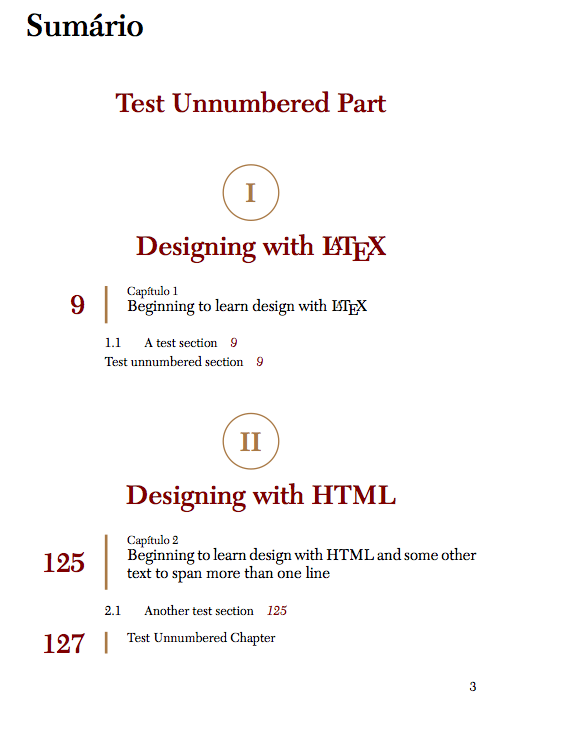
\includegraphics[width=0.8\textwidth]{sumario}
%\caption{Um exemplo de sumário}
%\label{exemplo-sumario}
%\end{figure}
%
%
%Naturalmente, também é possível mudar as cores no código.
%Os exemplos foram retirados de: \url{http://tex.stackexchange.com/questions/35825/pretty-table-of-contents} e modificados.




\chapter*{}
\phantom{}
\vfill
Este texto foi composto e adaptado (uma tradução livre com acréscimos) de: \url{http://en.wikibooks.org/wiki/LaTeX/}. Tipologia: Bulmer. A classe utilizada foi \KOMAScript{}.

\medskip

\ccbyncsa

\medskip
Os direitos desta obra são regidos pela licença \textbf{Creative Commons}. Sua distribuição e cópia é livre, desde que citada a fonte, e pode ser modificada, mas não utilizada para fins comerciais.  Ver: \url{http://creativecommons.org/licenses/by-nc-sa/3.0/br/}.

\end{document}


%Para mudar os dois pontos depois de Figura X:
%\newcommand*{\captionformat}{:\ } — este é o original
%\renewcommand*{\captionformat}{.\ } — este é "Figura X.”

%\usepackage[frenchchapters]{impnattypo}
%Para usar "Chapitre Premier" em vez de "Chapitre I" quando em francês.

